% !TeX spellcheck = hu_HU
% !TeX encoding = UTF-8
% !TeX program = xelatex
% TODO Change language to en_GB (recommended) or en_US for English documents
\documentclass[11pt,a4paper,oneside]{report}             % Single-side
%\documentclass[11pt,a4paper,twoside,openright]{report}  % Duplex

% thanks to http://tex.stackexchange.com/a/47579/71109
\usepackage{ifxetex}
\usepackage{ifluatex}
\newif\ifxetexorluatex % a new conditional starts as false
\ifnum 0\ifxetex 1\fi\ifluatex 1\fi>0
   \xetexorluatextrue
\fi

\ifxetexorluatex
  \usepackage{fontspec}
\else
  \usepackage[T1]{fontenc}
  \usepackage[utf8]{inputenc}
  \usepackage[lighttt]{lmodern}
\fi

\usepackage[english,magyar]{babel} % Alapértelmezés szerint utoljára definiált nyelv lesz aktív, de később külön beállítjuk az aktív nyelvet.

%\usepackage{cmap}
\usepackage{amsfonts,amsmath,amssymb} % Mathematical symbols.
%\usepackage[ruled,boxed,resetcount,linesnumbered]{algorithm2e} % For pseudocodes. % beware: this is not compatible with LuaLaTeX, see http://tex.stackexchange.com/questions/34814/lualatex-and-algorithm2e
\usepackage{booktabs} % For publication quality tables for LaTeX
\usepackage{graphicx}

%\usepackage{fancyhdr}
%\usepackage{lastpage}

\usepackage{anysize}
%\usepackage{sectsty}
\usepackage{setspace} % For setting line spacing

\usepackage[unicode]{hyperref} % For hyperlinks in the generated document.
\usepackage{xcolor}
\usepackage{listings} % For source code snippets.

\usepackage[amsmath,thmmarks]{ntheorem} % Theorem-like environments.

\usepackage[hang]{caption}

\singlespacing

\newcommand{\selecthungarian}{
	\selectlanguage{magyar}
	\setlength{\parindent}{2em}
	\setlength{\parskip}{0em}
	\frenchspacing
}

\newcommand{\selectenglish}{
	\selectlanguage{english}
	\setlength{\parindent}{0em}
	\setlength{\parskip}{0.5em}
	\nonfrenchspacing
	\renewcommand{\figureautorefname}{Figure}
	\renewcommand{\tableautorefname}{Table}
	\renewcommand{\partautorefname}{Part}
	\renewcommand{\chapterautorefname}{Chapter}
	\renewcommand{\sectionautorefname}{Section}
	\renewcommand{\subsectionautorefname}{Section}
	\renewcommand{\subsubsectionautorefname}{Section}
}

\usepackage[numbers]{natbib}
\usepackage{xspace}


%TODO Set the main variables
\newcommand{\vikszerzoVezeteknev}{Holló-Szabó}
\newcommand{\vikszerzoKeresztnev}{Ákos}

\newcommand{\vikkonzulensAMegszolitas}{}
\newcommand{\vikkonzulensAVezeteknev}{Ács}
\newcommand{\vikkonzulensAKeresztnev}{Evelin}

\newcommand{\vikkonzulensBMegszolitas}{dr.~}
\newcommand{\vikkonzulensBVezeteknev}{Nemeskey}
\newcommand{\vikkonzulensBKeresztnev}{Dávid}

\newcommand{\vikkonzulensCMegszolitas}{}
\newcommand{\vikkonzulensCVezeteknev}{}
\newcommand{\vikkonzulensCKeresztnev}{}

\newcommand{\vikcim}{Szemantikai elemzés gráf-transzformációkkal} % Cím
\newcommand{\viktanszek}{\bmemit} % Tanszék
\newcommand{\vikdoktipus}{\bsc} % Dokumentum típusa (\bsc vagy \msc)
\newcommand{\vikmunkatipusat}{szakdolgozatot} % a "hallgató nyilatkozat" részhez: szakdolgozatot vagy diplomatervet

%--------------------------------------------------------------------------------------
% TDK-specifikus változók
%--------------------------------------------------------------------------------------
\newcommand{\tdkszerzoB}{Második Szerző} % Második szerző neve; hagyd üresen, ha egyedül írtad a TDK-t.
\newcommand{\tdkev}{2014} % A dolgozat írásának éve (pl. "2014") (Ez OTDK-nál eltérhet az aktuális évtől.)

% További adatok az OTDK címlaphoz (BME-s TDK-hoz nem kell kitölteni)
\newcommand{\tdkevfolyamA}{IV} % Első szerző évfolyama, római számmal (pl. IV).
\newcommand{\tdkevfolyamB}{III} % Második szerző évfolyama, római számmal (pl. III).
\newcommand{\tdkkonzulensbeosztasA}{egyetemi tanár} % Első konzulens beosztása (pl. egyetemi docens)
\newcommand{\tdkkonzulensbeosztasB}{doktorandusz} % Második konzulens beosztása (pl. egyetemi docens)

\newcommand{\szerzoMeta}{\vikszerzoVezeteknev{} \vikszerzoKeresztnev} % egy szerző esetén
%\newcommand{\szerzoMeta}{\vikszerzoVezeteknev{} \vikszerzoKeresztnev, \tdkszerzoB} % két szerző esetén

%TODO Language configuration -- choose one
% Beállítások magyar nyelvű dolgozathoz
%%--------------------------------------------------------------------------------------
% Elnevezések
%--------------------------------------------------------------------------------------
\newcommand{\bme}{Budapesti Műszaki és Gazdaságtudományi Egyetem}
\newcommand{\vik}{Villamosmérnöki és Informatikai Kar}

\newcommand{\bmemit}{Méréstechnika és Információs Rendszerek Tanszék}

\newcommand{\keszitette}{Készítette}
\newcommand{\konzulens}{Konzulens}

\newcommand{\bsc}{Szakdolgozat}
\newcommand{\msc}{Diplomaterv}
\newcommand{\tdk}{TDK dolgozat}
\newcommand{\bsconlab}{BSc Önálló laboratórium}
\newcommand{\msconlabi}{MSc Önálló laboratórium 1.}
\newcommand{\msconlabii}{MSc Önálló laboratórium 2.}

\newcommand{\pelda}{Példa}
\newcommand{\definicio}{Definíció}
\newcommand{\tetel}{Tétel}

\newcommand{\bevezetes}{Bevezetés}
\newcommand{\koszonetnyilvanitas}{Köszönetnyilvánítás}
\newcommand{\fuggelek}{Függelék}

% Opcionálisan átnevezhető címek
%\addto\captionsmagyar{%
%\renewcommand{\listfigurename}{Saját ábrajegyzék cím}
%\renewcommand{\listtablename}{Saját táblázatjegyzék cím}
%\renewcommand{\bibname}{Saját irodalomjegyzék név}
%}

\newcommand{\szerzo}{\vikszerzoVezeteknev{} \vikszerzoKeresztnev}
\newcommand{\vikkonzulensA}{\vikkonzulensAMegszolitas\vikkonzulensAVezeteknev{} \vikkonzulensAKeresztnev}
\newcommand{\vikkonzulensB}{\vikkonzulensBMegszolitas\vikkonzulensBVezeteknev{} \vikkonzulensBKeresztnev}
\newcommand{\vikkonzulensC}{\vikkonzulensCMegszolitas\vikkonzulensCVezeteknev{} \vikkonzulensCKeresztnev}

\newcommand{\selectthesislanguage}{\selecthungarian}

\bibliographystyle{huplain}

\def\lstlistingname{lista}

\newcommand{\appendixnumber}{6}  % a fofejezet-szamlalo az angol ABC 6. betuje (F) lesz

% Settings for English documents
%--------------------------------------------------------------------------------------
% Elnevezések
%--------------------------------------------------------------------------------------
\newcommand{\bme}{Budapest University of Technology and Economics}
\newcommand{\vik}{Faculty of Electrical Engineering and Informatics}

\newcommand{\bmemit}{Department of Measurement and Information Systems}

\newcommand{\keszitette}{Author}
\newcommand{\konzulens}{Advisor}

\newcommand{\bsc}{Bachelor's Thesis}
\newcommand{\msc}{Master's Thesis}
\newcommand{\tdk}{Scientific Students' Association Report}
\newcommand{\bsconlab}{BSc Project Laboratory}
\newcommand{\msconlabi}{MSc Project Laboratory 1}
\newcommand{\msconlabii}{MSc Project Laboratory 2}

\newcommand{\pelda}{Example}
\newcommand{\definicio}{Definition}
\newcommand{\tetel}{Theorem}

\newcommand{\bevezetes}{Introduction}
\newcommand{\koszonetnyilvanitas}{Acknowledgements}
\newcommand{\fuggelek}{Appendix}

% Optional custom titles
%\addto\captionsenglish{%
%\renewcommand*{\listfigurename}{Your list of figures title}
%\renewcommand*{\listtablename}{Your list of tables title}
%\renewcommand*{\bibname}{Your bibliography title}
%}

\newcommand{\szerzo}{\vikszerzoKeresztnev{} \vikszerzoVezeteknev}
\newcommand{\vikkonzulensA}{\vikkonzulensAMegszolitas\vikkonzulensAKeresztnev{} \vikkonzulensAVezeteknev}
\newcommand{\vikkonzulensB}{\vikkonzulensBMegszolitas\vikkonzulensBKeresztnev{} \vikkonzulensBVezeteknev}
\newcommand{\vikkonzulensC}{\vikkonzulensCMegszolitas\vikkonzulensCKeresztnev{} \vikkonzulensCVezeteknev}

\newcommand{\selectthesislanguage}{\selectenglish}

\bibliographystyle{plainnat}

\newcommand{\ie}{i.e.\@\xspace}
\newcommand{\Ie}{I.e.\@\xspace}
\newcommand{\eg}{e.g.\@\xspace}
\newcommand{\Eg}{E.g.\@\xspace}
\newcommand{\etal}{et al.\@\xspace}
\newcommand{\etc}{etc.\@\xspace}
\newcommand{\vs}{vs.\@\xspace}
\newcommand{\viz}{viz.\@\xspace} % videlicet
\newcommand{\cf}{cf.\@\xspace} % confer
\newcommand{\Cf}{Cf.\@\xspace}
\newcommand{\wrt}{w.r.t.\@\xspace} % with respect to
\newcommand{\approximately}{approx.\@\xspace}

\newcommand{\appendixnumber}{1}  % a fofejezet-szamlalo az angol ABC 1. betuje (A) lesz


%--------------------------------------------------------------------------------------
% Page layout setup
%--------------------------------------------------------------------------------------
% we need to redefine the pagestyle plain
% another possibility is to use the body of this command without \fancypagestyle
% and use \pagestyle{fancy} but in that case the special pages
% (like the ToC, the References, and the Chapter pages)remain in plane style

\pagestyle{plain}
\marginsize{35mm}{25mm}{15mm}{15mm}

\setcounter{tocdepth}{3}
%\sectionfont{\large\upshape\bfseries}
\setcounter{secnumdepth}{3}

\sloppy % Margón túllógó sorok tiltása.
\widowpenalty=10000 \clubpenalty=10000 %A fattyú- és árvasorok elkerülése
\def\hyph{-\penalty0\hskip0pt\relax} % Kötőjeles szavak elválasztásának engedélyezése


%--------------------------------------------------------------------------------------
% Setup hyperref package
%--------------------------------------------------------------------------------------
\hypersetup{
    % bookmarks=true,            % show bookmarks bar?
    unicode=true,              % non-Latin characters in Acrobat's bookmarks
    pdftitle={\vikcim},        % title
    pdfauthor={\szerzoMeta},    % author
    pdfsubject={\vikdoktipus}, % subject of the document
    pdfcreator={\szerzoMeta},   % creator of the document
    pdfproducer={},    % producer of the document
    pdfkeywords={},    % list of keywords (separate then by comma)
    pdfnewwindow=true,         % links in new window
    colorlinks=true,           % false: boxed links; true: colored links
    linkcolor=black,           % color of internal links
    citecolor=black,           % color of links to bibliography
    filecolor=black,           % color of file links
    urlcolor=black             % color of external links
}


%--------------------------------------------------------------------------------------
% Set up listings
%--------------------------------------------------------------------------------------
\definecolor{lightgray}{rgb}{0.95,0.95,0.95}
\lstset{
	basicstyle=\scriptsize\ttfamily, % print whole listing small
	keywordstyle=\color{black}\bfseries, % bold black keywords
	identifierstyle=, % nothing happens
	% default behavior: comments in italic, to change use
	% commentstyle=\color{green}, % for e.g. green comments
	stringstyle=\scriptsize,
	showstringspaces=false, % no special string spaces
	aboveskip=3pt,
	belowskip=3pt,
	backgroundcolor=\color{lightgray},
	columns=flexible,
	keepspaces=true,
	escapeinside={(*@}{@*)},
	captionpos=b,
	breaklines=true,
	frame=single,
	float=!ht,
	tabsize=2,
	literate=*
		{á}{{\'a}}1	{é}{{\'e}}1	{í}{{\'i}}1	{ó}{{\'o}}1	{ö}{{\"o}}1	{ő}{{\H{o}}}1	{ú}{{\'u}}1	{ü}{{\"u}}1	{ű}{{\H{u}}}1
		{Á}{{\'A}}1	{É}{{\'E}}1	{Í}{{\'I}}1	{Ó}{{\'O}}1	{Ö}{{\"O}}1	{Ő}{{\H{O}}}1	{Ú}{{\'U}}1	{Ü}{{\"U}}1	{Ű}{{\H{U}}}1
		{Ű}{{\Σ{Σ}}}1
}


%--------------------------------------------------------------------------------------
% Set up theorem-like environments
%--------------------------------------------------------------------------------------
% Using ntheorem package -- see http://www.math.washington.edu/tex-archive/macros/latex/contrib/ntheorem/ntheorem.pdf

\theoremstyle{plain}
\theoremseparator{.}
\newtheorem{example}{\pelda}

\theoremseparator{.}
%\theoremprework{\bigskip\hrule\medskip}
%\theorempostwork{\hrule\bigskip}
\theorembodyfont{\upshape}
\theoremsymbol{{\large \ensuremath{\centerdot}}}
\newtheorem{definition}{\definicio}

\theoremseparator{.}
%\theoremprework{\bigskip\hrule\medskip}
%\theorempostwork{\hrule\bigskip}
\newtheorem{theorem}{\tetel}


%--------------------------------------------------------------------------------------
% Some new commands and declarations
%--------------------------------------------------------------------------------------
\newcommand{\code}[1]{{\upshape\ttfamily\scriptsize\indent #1}}
\newcommand{\doi}[1]{DOI: \href{http://dx.doi.org/\detokenize{#1}}{\raggedright{\texttt{\detokenize{#1}}}}} % A hivatkozások közt így könnyebb DOI-t megadni.

\DeclareMathOperator*{\argmax}{arg\,max}
%\DeclareMathOperator*[1]{\floor}{arg\,max}
\DeclareMathOperator{\sign}{sgn}
\DeclareMathOperator{\rot}{rot}


%--------------------------------------------------------------------------------------
% Setup captions
%--------------------------------------------------------------------------------------
\captionsetup[figure]{
	width=.75\textwidth,
	aboveskip=10pt}

\renewcommand{\captionlabelfont}{\bf}
%\renewcommand{\captionfont}{\footnotesize\it}

%--------------------------------------------------------------------------------------
% Hyphenation exceptions
%--------------------------------------------------------------------------------------
\hyphenation{Shakes-peare Mar-seilles ár-víz-tű-rő tü-kör-fú-ró-gép}


\author{\vikszerzo}
\title{\viktitle}

%--------------------------------------------------------------------------------------
% Table of contents and the main text
%--------------------------------------------------------------------------------------
\begin{document}

\pagenumbering{gobble}

%TODO These includes define guidelines -- remove these
%~~~~~~~~~~~~~~~~~~~~~~~~~~~~~~~~~~~~~~~~~~~~~~~~~~~~~~~~~~~~~~~~~~~~~~~~~~~~~~~~~~~~~~
%--------------------------------------------------------------------------------------
% Feladatkiiras (a tanszeken atveheto, kinyomtatott valtozat)
%--------------------------------------------------------------------------------------
\clearpage
\begin{center}
\large
\textbf{FELADATKIÍRÁS}\\
\end{center}

A feladatkiírást a tanszéki adminisztrációban lehet átvenni, és a leadott munkába eredeti, tanszéki pecséttel ellátott és a tanszékvezető által aláírt lapot kell belefűzni (ezen oldal \emph{helyett}, ez az oldal csak útmutatás). Az elektronikusan feltöltött dolgozatban már nem kell beleszerkeszteni ezt a feladatkiírást.


\selectthesislanguage

%TODO Titlepage -- choose one from below
%~~~~~~~~~~~~~~~~~~~~~~~~~~~~~~~~~~~~~~~~~~~~~~~~~~~~~~~~~~~~~~~~~~~~~~~~~~~~~~~~~~~~~~
%--------------------------------------------------------------------------------------
%	The title page
%--------------------------------------------------------------------------------------
\begin{titlepage}
\begin{center}

\includegraphics[width=60mm,keepaspectratio]{figures/BMElogo.png}\\
\vspace{0.3cm}
\textbf{Budapesti M�szaki �s Gazdas�gtudom�nyi Egyetem}\\
\textmd{Villamosm�rn�ki �s Informatikai Kar}\\
\textmd{\viktanszek}\\[5cm]

\vspace{0.4cm}
{\huge \bfseries \vikcim}\\[0.8cm]
\vspace{0.5cm}
\textsc{\Large \vikdoktipus}\\[4cm]

\begin{tabular}{cc}
 \makebox[7cm]{\emph{K�sz�tette}} & \makebox[7cm]{\emph{Konzulens}} \\
 \makebox[7cm]{\vikszerzo} & \makebox[7cm]{\vikkonzulens}
\end{tabular}

\vfill
{\large \today}
\end{center}
\end{titlepage}


		   % Szakdolgozat/Diplomaterv címlap
%%% TDK címlap
\begin{titlepage}
  \begin{center}  
  
\includegraphics[width=7cm]{./figures/bme_logo.pdf}
  \vspace{0.3cm}
  
  \bme \\
  \vik \\
  \viktanszek \\
  \vspace{5cm}
  
  \huge {\vikcim}
  \vspace{1.5cm}
  
  \large {\textbf{\tdk}}
  \vfill
    
  {\Large 
  	\keszitette: \\ \vspace{0.3cm}
  	\szerzo \\
	\tdkszerzoB \\
  	\vspace{1.5cm}
  	\konzulens: \\ \vspace{0.3cm}
  	\vikkonzulensA \\
  	\vikkonzulensB \\
  }
  
  \vspace{2cm}
  \large {\tdkev}
 \end{center}
\end{titlepage}
%% Címlap vége
	% TDK címlap
%%% OTDK külső címlap
\begin{titlepage}
  	$\;$ 
	\vspace{5cm}
	
	\begin{center}
	\Huge
	\textbf{TDK-dolgozat}\let\thefootnote\relax\footnote{A dolgozat bemutatását a XXXXXXXXX  ``Lorem ipsum dolor sit amet'' című program támogatta.}
	\end{center}
	
	\vspace{13cm}
	
	\Large
	\hspace{8cm} \szerzo
	
	\hspace{8cm} \tdkszerzoB
	
	\hspace{8cm} \tdkev.
\end{titlepage}

\newpage
\thispagestyle{empty}


%% OTDK belső címlap
\begin{titlepage}
  \begin{center}  
  
\includegraphics[width=7cm]{./figures/bme_logo.pdf}
  \vspace{0.3cm}
  
  \bme \\
  \vik \\
  \viktanszek \\
  \vspace{3.5cm}
  
  \huge {\vikcim}
  \vspace{1.5cm}
  
  \large {\textbf{\vikdoktipus}}
  \vfill
    
  {\Large 
  	{\large \keszitette:} \\ \vspace{0.2cm}
  	\szerzo \\ \tdkevfolyamA. évfolyam \\
	\vspace{0.5cm}
	\tdkszerzoB \\ \tdkevfolyamB. évfolyam \\
  	\vspace{1.5cm}
  	{\large \konzulens:} \\ \vspace{0.2cm}
  	\vikkonzulensA,\\ \tdkkonzulensbeosztasA \\
  	\vspace{0.5cm}
  	\vikkonzulensB,\\ \tdkkonzulensbeosztasB \\
  }
  
  \vspace{2cm}
  \large {\tdkev.}
  
 \end{center}
\end{titlepage}   % OTDK címlap


% Table of Contents
%~~~~~~~~~~~~~~~~~~~~~~~~~~~~~~~~~~~~~~~~~~~~~~~~~~~~~~~~~~~~~~~~~~~~~~~~~~~~~~~~~~~~~~
\tableofcontents\vfill


% Declaration and Abstract
%~~~~~~~~~~~~~~~~~~~~~~~~~~~~~~~~~~~~~~~~~~~~~~~~~~~~~~~~~~~~~~~~~~~~~~~~~~~~~~~~~~~~~~
%--------------------------------------------------------------------------------------
% Nyilatkozat
%--------------------------------------------------------------------------------------
\begin{center}
\large
\textbf{HALLGAT�I NYILATKOZAT}\\
\end{center}

Alul�rott \emph{\vikszerzo}, szigorl� hallgat� kijelentem, hogy ezt a szakdolgozatot/ diplomatervet \textcolor{blue}{(nem k�v�nt t�rlend�)} meg nem engedett seg�ts�g n�lk�l, saj�t magam k�sz�tettem, csak a megadott forr�sokat (szakirodalom, eszk�z�k stb.) haszn�ltam fel. Minden olyan r�szt, melyet sz� szerint, vagy azonos �rtelemben, de �tfogalmazva m�s forr�sb�l �tvettem, egy�rtelm�en, a forr�s megad�s�val megjel�ltem.

Hozz�j�rulok, hogy a jelen munk�m alapadatait (szerz�(k), c�m, angol �s magyar nyelv� tartalmi kivonat, k�sz�t�s �ve, konzulens(ek) neve) a BME VIK nyilv�nosan hozz�f�rhet� elektronikus form�ban, a munka teljes sz�veg�t pedig az egyetem bels� h�l�zat�n kereszt�l (vagy autentik�lt felhaszn�l�k sz�m�ra) k�zz�tegye. Kijelentem, hogy a beny�jtott munka �s annak elektronikus verzi�ja megegyezik. D�k�ni enged�llyel titkos�tott diplomatervek eset�n a dolgozat sz�vege csak 3 �v eltelte ut�n v�lik hozz�f�rhet�v�.

\begin{flushleft}
\vspace*{1cm}
Budapest, \today
\end{flushleft}

\begin{flushright}
 \vspace*{1cm}
 \makebox[7cm]{\rule{6cm}{.4pt}}\\
 \makebox[7cm]{\emph{\vikszerzo}}\\
 \makebox[7cm]{hallgat�}
\end{flushright}
\thispagestyle{empty}

\vfill
\clearpage
\thispagestyle{empty} % an empty page

 %TODO Hallgatói nyilatkozat -- TDK és OTDK esetén törlendő!
%----------------------------------------------------------------------------
% Abstract in hungarian
%----------------------------------------------------------------------------
\chapter*{Kivonat}\addcontentsline{toc}{chapter}{Kivonat}

Jelen dokumentum egy diplomaterv sablon, amely formai keretet ad a BME Villamosm�rn�ki �s Informatikai Kar�n v�gz� hallgat�k �ltal elk�sz�tend� szakdolgozatnak �s diplomatervnek. A sablon haszn�lata opcion�lis. Ez a sablon \LaTeX~alap�, a \emph{TeXLive} \TeX-implement�ci�val �s a PDF-\LaTeX~ford�t�val m�k�d�k�pes.
\vfill

%----------------------------------------------------------------------------
% Abstract in english
%----------------------------------------------------------------------------
\chapter*{Abstract}\addcontentsline{toc}{chapter}{Abstract}

This document is a \LaTeX-based skeleton for BSc/MSc~theses of students at the Electrical Engineering and Informatics Faculty, Budapest University of Technology and Economics. The usage of this skeleton is optional. It has been tested with the \emph{TeXLive} \TeX~implementation, and it requires the PDF-\LaTeX~compiler.
\vfill

    %TODO Összefoglaló -- TDK és OTDK esetén nem kötelező


% The main part of the thesis
%~~~~~~~~~~~~~~~~~~~~~~~~~~~~~~~~~~~~~~~~~~~~~~~~~~~~~~~~~~~~~~~~~~~~~~~~~~~~~~~~~~~~~~
\pagenumbering{arabic}

%TODO import your own content
%----------------------------------------------------------------------------
\chapter{Bevezetés}
%----------------------------------------------------------------------------

Manapság egyre több technológia jelenik meg, aminek alapja az NLP (Natural Language Processing). Ezek a technológiák nagy része nem lenne megvalósítható szemantikai elemzés nélkül. A szemantikai elemzés célja, hogy egy nyers szövegből, vagy beszédhangból előállítsa annak a szemantikai reprezentációját. Ez a reprezentáció egy irányított gráf is lehet, amit ha a mondat szintaktikai szerkezetét reprezentáló fákból állítunk elő, akkor a teljes feladat felfogható egy gráf-transzformációként. 

Bár szemantikai elemzésre számos Deep Learning-es megoldás létezik, ezek pontatlansága nagy igényt teremt egy analitikus mély szemantikai elemzési módszerre. A gráf transzformációs megközelítés ígéretes eredményeket mutatott fel, mint például a Stanford Parser, ami TREGEX-ek segítségével végzi el tiszta analitikus módon a transzformációkat.
Több formalizmus is létezik a transzformációk leírására, mint például a HRG (hyperedge-replacement grammar) vagy az IRTG(interpreted regular tree grammars). Jelenleg is egy ezekkel kapcsolatos kutatás folyik az AUT tanszéken.

A kutatás során az ALTO(Algebraic Language Toolkit)-val dolgoztunk, ami a jelenlegi leghatékonyabb környezet IRTG-k futtatására. Ugyanakkor a kutatásnak állandó gátját jelenti, hogy az IRTG még egy fejletlen nyelvtan és nehezen átlátható; és az ALTO-ból is hiányoznak fontos funkcionalitások. A problémán sokat enyhítene, ha az IRTG szabályokat REGEX-ek segítségével is meglehetne hivatkozni.

Szakdolgozatom keretében egy templatelésre alkalmas nyelvet fejlesztettem ki, ami a Slime fantázianévre hallgat. Segítségével az IRTG nyelvtanokat tömörebben és átláthatóbban lehet definiálni. Mivel az ALTO java-ban készül, a nyelv Kotlinban készül ANTLRv4 segítségével. Még nincs teljesen kifejlődve, de a feladathoz szükséges megoldásokat tartalmazza. Ilyen például a template definiálás, egymásba ágyazás, regexxel hivatkozás és sok egyéb. Teljes formájában egy univerzális bővítmény lesz, ami bármely nyelv vagy szöveg felett használható.
 	 	 	
A dolgozat a következőképpen épül fel: Az 1. fejezetben bemutatom a …., a 2. fejezetben a ….-ról írok, majd a 3. fejezetben a …., végül ….

%----------------------------------------------------------------------------
\chapter{Szemantikai elemzés gráf-transzformációkkal}
\label{sec:SemParsWithGraphTrans}
%----------------------------------------------------------------------------
\section{Szintaxis}
%----------------------------------------------------------------------------
Egy nyelv jelentéstől független struktúráját nevezzük szintaxisnak. Szintaxis-ról beszélhetünk természetes nyelvek és programozási nyelvek esetén is. Ide tartozik, hogy a szöveg hogyan bomlik eltérő szerepű szavakra és jelekre [Nem kell, de miért jelennek meg a stanford fákban? a penn treebank egy korpusz, és valahogy kezelni akarták az írásjeleket, így döntöttek az annotátorok, de a nyelvészetben az írásjel nem a konstituens része, látni fogod majd, ha elolvasod az idevágó irodalmakat, amiket küldtem] és hogy ezek milyen hierarchikus rendszert alkotnak. A nyelvészetben a konstituens fa, avagy szintaktikai fa reprezentálja a szöveg szintaxisát, ami a tokeneket kifejezésekbe, majd mondatrészekbe és mondatokba rendezi. [hm, ez szerintem kissé pontatlan, megkérdezem a Gábort, hogy szerinte hogyan lehetne jobban] Az NLP-ben e helyett a függőségi gráfok terjedtek el, amik a szavak között címkézett irányított élekből építenek egy irányított gráfot. Ebben a fejezetben ezt a két formalizmust fejtem ki részletesebben.

%----------------------------------------------------------------------------
\subsection{A Szintaktikai Fa}
%----------------------------------------------------------------------------
A nyelvészet szemlélete szerint bármelyik emberi nyelv szintaxisa leírható egy Környezetfüggetlen Nyelvtannal.

Környezet Független Nyelvtannak egy $G=(N,\sum ,P,S)$ rendezett négyest nevezünk, ahol:

\begin{itemize}
	\item \emph{$N$} nemterminális ábécé
	\item \emph{$\Sigma$} terminális ábécé amire $ N \cap \Sigma =\varnothing $
	\item \emph{$S\in N$} a kezdőszimbólum
	\item \emph{$P$} pedig $\alpha \to \beta$ alakú átjárási szabályok véges halmaza, ahol $\alpha,\beta \in(N \cup \Sigma)*$ és $\alpha$ -ban van legalább egy nemterminális betű.
\end{itemize}
$https://people.inf.elte.hu/kubuaai/FoNYa/formalis_nyelvek_kidolgozott_tetelek.pdf[ másik forrást]$
Ebben a nyelvtanban a terminális szimbólumok a szavak és az azokat tagoló írásjelek. A nemterminális szimbólumok három szintre sorolhatóak. A legalsó szint a szavak szintje, ahova a szófajokat és írásjel[kell-e?] [írásjel alapjáraton nem kell szerintem; a mi nyelvtanunk a penn treebank sajátosságai miatt kezeli ugyan] kategóriákat jelölő csúcsok tartoznak. Ezek a csúcsok átírásával közvetlen a terminális szimbólumokat kapjuk. A terminális szimbólumokat eredményező átírási szabályokat “terminális szabály”-oknak hívják. A második szint a kifejezések szintje, ahova a szavak alkotta kifejezéseket jelölő (nagyjából 20 féle) csúcsok tartoznak . Ezek a csúcsok írhatóak át a típusuknak megfelelő headerű kifejezésekké, amik további kifejezésekből és szavakból állnak. A harmadik szint a mondatrészek szintje, amihez a mondat egészét jelölő ‘S’(sentance) és a mondatrészeket jelölő négy további szimbólum tartoznak.  A kezdő karakter az S, mint “sentence”. Egy mondat akkor helyes szintaktikailag, ha létezik a környezetfüggetlen nyelvtanban levezetése. Ha létezik levezetése, akkor a levezetési fa maga a mondat Szintaktikai Fája.

Ezek például a 2.2.4-es pontban található szintaktikai fa szabályai

( a “John loves Mary.” mondaté: 

S3( NP1( NNP( John ) ), VP2( VBZ( loves ),  NP1( NNP( Mary ) ) ), .( . ) ) ) :
\begin{itemize}
\item$S \to NP VP$ .
\item$NP \to NNP$
\item$VP \to VBZ NP$
\item$NNP \to John | Mary$
\item$VBZ \to loves$
\item$. \to .$
\end{itemize}

A szintaktikai fa a legbevettebb reprezentációja a mondatok szintaxisának a nyelvészetben. Analitikus megközelítés esetén is legtöbbször a szintaktikai fa az első, amit elkészítünk. Ehhez először a szavakat feltokenezzük, avagy meghatározzuk a terminális szimbólumok határait és kigeneráljuk a megfelelő “szófaj token”-t mindegyikhez. Végezetül megkeressük valószínűségi súlyozásokkal gyorsítva a legvalószínűbb levezetését az adott nyelv átírási szabályai alapján.


%----------------------------------------------------------------------------
\subsection{UD és a dependencia elemzés}
%----------------------------------------------------------------------------
A dependencia alapú megközelítés szerint a szintaktikai szerkezet lexikai elemekből áll, amiket bináris kapcsolatok kötnek össze. A dependencia fogalma azt jelenti, hogy a szavak(fej és dependens) irányított kapcsolatokkal vannak összekötve.  Általában az állítmány a gráf gyökércsomópontja vagy a strukturális középpontja a mondatnak. A mondat szerkezetét a fejek és dependensek közötti viszonyok adják. Sok jól ismert elmélete van a függőségi nyelvtanoknak, összefoglalásért lásd (Nivre, 2005, p.  3).

Az UD(Universal Dependency) [UD weboldalát, (De Marneffe et al. (2014))] információt egy DAO gráfon szemlélteti, aminek csúcsai a szavak, és élei pedig a szavak közötti viszonyok. Az UD-hez hasonló Függőségi Gráfoknak sok féle formalizmusa létezik. Az NLP területén ezt a reprezentációt használják legtöbbször a szintaxis reprezentálására. Mi a kutatásunk során az UD-t használtuk.

Az UD projekt egy nyelvek közötti konzisztens annotációs rendszer és fa adatbázis hatvannál is több nyelvre. Kategóriák és annotációk univerzális készletét nyújtja miközben miközben megenged nyelvfüggő kiterjesztéseket is. A szavak közötti nyelvtani viszonyt szemlélteti, mint például az alany-állítmányi vagy tárgy-állítmányi vagy jelzői. Az UD a Stanford Dependencies [hivatkozás: (De Marneffe and Manning (2008)] fejlődött ki, amit egyesítettek a Google univerzális címkékkel [Petrov et al. (2011)], az “Interset feature inventory”-nak egy átdolgozott rész halmazával [Zeman (2008)] és  a CoNLL-X formátum egy átdolgozott verziójával [Buchholz and
Marsi (2006)].

[példaelemzést LaTexben]

Az alap függőségek két csoportba sorolhatóak. Az egyik csoport a klauzális (“clausal”) viszonyok, amik szintaktikai szerepeket írnak le a predikátumra vonatkozóan. A másik csoport a módosító viszonyok, amik azt írják le, hogy a fejet hogyan módosítja a függőben lévő szó. (Jurafsky and Martin (2018b)) Az egységes analízis okán a függőségek fejének a főnevet tekintjük, amit bemutat egy elöljáró vagy van hozzá csatlakozó. Más esetben a jelölőt tekintjük a függőség fejének. A formalizmus egy lexikalista megközelítést követ a számítás beli használat megvalósítására: a szintaktikai szerkezetek  lexikai elemekből állnak, amik aszimmetrikus egy az egyhez kapcsolatokkal vannak összekötve a hatókörrel ellentétben, ami egy egy a többhöz kapcsolat.  [De Marneffe et al. (2014)]Az UD lehetővé teszi dependencia parszerek nyelveken keresztüli kiértékelését. Több mint 30 csapat vett részt 2017-ben a közös céllal, hogy megvalósítsák a többnyelvű dependencia elemzést [shared taskos papert hivatkozd 2018].

szavak közötti viszonyok, angolul és jelölésük:
[(Jurafsky and Martin, 2018b, p. 3)]

[itt meg lehetne olyan alfejezet, hogy “Szemantika”
írhatnád benne, hogy mi az a szemantikai elemzés, hogy lehet csinálni (shallow vs. deep, vektorterek vs. gráfos cucc), de az ilyen átvezető részeket segítek majd megírni, vagyis átírok majd egyet-kettőt, ha megírtad, de olyasmik legyenek, mint a szakdolgozatomban amik vannak]


%----------------------------------------------------------------------------
\section{4lang}
%----------------------------------------------------------------------------
A 4lang  [(Kornai et al. (2015))] egy formalizmus, ami irányított gráfokat épít szemantikai reprezentáció céljával. A gráfban a csúcsok nem szavakat, hanem nyelvfüggetlen fogalmakat jelölnek. Ezeknek a fogalmaknak már nincsenek nyelvtani jellemzőik és a kompetens beszélők közös tudását reprezentálja a fogalomról. Például a fagy[ \texttt{fagy}] mit főnév vagy ige vagy fagyás vagy fagyott szava nincsenek megkülönböztetve a 4lang reprezentációban [itt hivatkozzuk, akinél ezt a példát először olvastuk] Ezáltal a 4lang fogalmak és a nekik egy nyelvben megfelelő szavak között egy a többhöz kapcsolat áll fenn.

A csúcsokat három féle él kapcsolhatja össze:
0-él reprezentálja a tulajdonságokat. Például $virág -0-> szép$, az $AZ\_EGY$($IS\_A$) viszony $virág -0->  növény$ és unáris predikció $virág -0-> bimbózás$.
1 és 2-élek bináris predikciókat kapcsolnak az argumentumaikhoz. Például $James <-1- szeretet -2> kutya$.
Binary (tranzitív) elemek, amik nem felelnek meg egyik szónak sem egy kifejezésben vagy mondatban, NAGY BETŰS nyomtatott nevekkel vannak jelölve.

Létezik egy másik él konfiguráció is, ami megjelenhet 4lang gráfban, $w_1 <-0-1-> w_2$ . Erre azért van szükség, hogy konzisztensen lehessen jelölni a tárgy és predikátum közötti viszonyt. Vegyük például a “I’am writing.”(“Én éppen írok”)  mondatot az $i -0> write$ 4lang gráffal és az “I’am writing a letter”(“Én egy levelet írok éppen”) mondatot az $i <-1- write -2-> letter$ gráffal . Ez a két példa a dupla él nélkül azt jelentené, hogy a két az “i” és a “write” között attól függ a viszony, hogy adott e a tárgy vagy sem. [Recski (2018)]

A 4lang könyvtár tartalmaz eszközöket, amelyek képesek 4lang gráfokat építeni Nyers Szövegből és Szótári definíciókból (text\_ to\_ 4lang, dict\_ to\_ 4lang). A mag modulja a 4lang könyvtárnak, dep\_ to\_ 4lang, 4lang viszonyokat nyer ki szövegből, a Stanford Parser [DeMarneffe et al. (2006)] kimenetének a feldolgozásával és a Stanford függőségeknek a leképzésével 4lang részfáká.
4lang a neve egy kézzel alkotott  fogalmi szótárnak is, ami négy nyelven tartalmazza nyelvfüggetlen fogalmak több mint 2000 definícióját (magyar, angol, latin, lengyel). [Kornai and Makrai (2013)]
[ezt majd lehet hogy átrendezzük másik alpont alá, de amit írsz, az tök oké]


%----------------------------------------------------------------------------
\section{A 4lang és az UD különbségei}
%----------------------------------------------------------------------------
A munkánk során mint majd alaposabban is bemutatom a nyelvtan generálásánál, alaposan kihasználtuk a 4lang és az UD közötti hasonlóságot. Mindkét esetében egy irányított gráfról beszélünk. Mindkét esetében a csúcsok megfeleltethetőek a szavaknak, és az élek szavak közötti viszonyokat jelölik. Maguk a függőségek is sok esetben megfeleltethetőek egymásnak. Például a $w_1 -amod-> w_2$ viszony az UD-ból megfelel a $w_1 -0-> w_2$ viszonynak a 4lang-ból.

A kettő között ugyanakkor fontos elméleti és jelölésbeli különbségek vannak. Az UD a mondatok szintaxisát reprezentálja, míg a 4lang a szemantikai jelentését. Az UD-ben a csúcsok maguk a szavak, míg 4lang-ban a szavaknak megfeleltethető fogalmak. Az UD élei a szavak közötti nyelvtani viszonyt jelölik, addig a 4lang élek a szavak közötti szemantikai függőségekket. A 4lang függőségek és az UD függőségek között egy a többhöz viszony áll fenn, ahogy a szavak, és a 4lang beli fogalmak között is. Ez persze azt jelenti, hogy az UD már tartalmazza a szemantikára vonatkozó információkat is, de csak közvetetten.

[UD-4lang megfeleltetéses táblázat]

Bár a mondat UD gráfjából a 4lang gráfja levezethető, a két formalizmus tartalma mégsem ekvivalens. A 4lang gráfból már nem mindig vezethető le egyértelműen az UD. Az UD szavairól pedig nem egyértelmű, hogy a 4lang mely fogalmaira vetítsük le őket. A több jelentéső szavak is nehezítik a helyzetet, mivel ekkor a szónak megfelelő fogalom már függ a szó környezetétől is. A projekt jelenlegi fázisában még nem foglalkoztunk a szavak és 4lang fogalmak megfeleltetésével. Még nem áll rendelkezésünkre erre automatikus módszer. Mivel egy nyelv szókészlete és szavainak jelentése is állandóan változik, teljsen elvetendő a a megfeleltetésekhez szükséges adatok manuális előállítása.



%----------------------------------------------------------------------------
\section{A kutatás célja}
%----------------------------------------------------------------------------


A kutatásunk célja az, hogy a nyers szöveg és a feljebb leírt interpretációk bármelyikéből le tudjuk a többit generálni. Ha az egyik interpretációhoz a másikból több is tartozik, akkor képesek akarunk lenni az összes verziót legenerálni és a legalkalmasabbat automatikusan kiválasztani valószínűségi súlyozás segítségével. Minél kevesebb nyelvet szeretnénk használni, és minél kevesebb módszertant. Ez utóbbi szemponttól azt várjuk, hogy könnyebb lesz a kódot karbantartani és bővíteni további interpretációkkal. Mind ezt hatékonyan is szeretnénk csinálni. E téren az alap célunk egy négyzetes lefutási idő a bemenet méretének függvényében. Ezeknek a megkötéseknek az IRTG nyelv eleget tesz. Hiszen nagyon eltérő interpretációk esetében is legfeljebb interpretációk száma plusz egy nyelvet kell használnunk. Ugyanakkor, ha kiegészítjük az IRTG-t egy összetettebb gráf algebrával, az képes lehet minden interpretáció hatékony leírására és mindehhez két nyelvet kellene használnia.

%----------------------------------------------------------------------------
\section{Az IRTG és az alárendelt algebrák}
%----------------------------------------------------------------------------
Ebben a fejezetben a kutatás során használt környezetről(ALTO), formalizmusról(IRTG), algebrákról(SA,TTA,SGA), hátrányaikról és az ezeket kiküszöbölő ideiglenes megoldásainkról lesz szó.


%----------------------------------------------------------------------------
\subsection{Az ALTO}
%----------------------------------------------------------------------------
A kutatás során a kódot az Algebraic Language Toolkit-tel, avagy ALTO-val fordítjuk és futtatjuk. Az ALTO egy nyílt forrású parszer, ami többféle algebrát is megvalósít, ami IRTG-be ágyazva használható.
Ezek egyike az s-graph és a tag tree algebra. Ezen kívül is szabadon bővíthető új algebrákkal. Már korábban is használták gráf transzformációra és szemantikai feldolgozásra is. Nagy előnyt jelent, hogy Java-ban lett implementálva , így szinte bármely platformon futtatható. Ezen kívül rendelkezik grafikus és konzolos felhasználói felülettel is.


%----------------------------------------------------------------------------
\subsection{Az IRTG}
%----------------------------------------------------------------------------
Az IRTG (Interpreted Regular Tree Grammar, Interpretált Reguláris Fa Nyelvtan) egy kontextusfüggetlen nyelvtan, ami egy vagy több algebrába beágyazott újraíró szabályokból áll.
\begin{verbatim}
NP -> _NP2_amod_JJ_NN(JJ, NN)
[string] *(?1,?2)
[tree] NP2(?1, ?2)
[ud] merge(f_dep(merge("(r<root> :amod (d<dep>))", r_dep(?1))),?2)
[fourlang] merge(f_dep(merge("(r<root> :0 (d<dep>))", r_dep(?1))),?2)
\end{verbatim}

1. ábra: Egy, a amod relációt leíró IRTG-szabály négy algebrával

A szabálysorok egy környezetfüggetlen nyelvtan átírási szabályait adják meg. A szabályok feldolgozásakor először egy levezetési fa (derivation tree) épül, amelyek a nonterminálisokat lecserélő szabályokat tartalmazzák. Egy szabályt a következő módon lehet definiálni (a sablonban a változó részeket \{\$ \$\}zárójellel jelöltem, ahol a \$ a Slot kifejezésből ered, a \{\} pedig a nem szöveg elemeket jelöli):
\begin{verbatim}
[{$ interpretáció neve $}] {$ interpretáció lépése $}
\end{verbatim}
A interpretációk nyelve és kimenete többféle is lehet.  Választható például a szöveg kimenetű String Algebra, a csúcs sorrendet tartó fa gráf kimenetű Tag Tree Algebra, vagy  az irányított gráf kimenetű S-graphAlgebra. Az algebrák és az interpretációk között egy a többhöz kapcsolat van. Az interpretációk egymástól teljesen függetlenek. Egy szabályban minden interpretációt meg kell adni. Minden átírás során, minden interpretációra vonatkozó derivációba beszúródnak az alkalmazott szabályban az interpretációhoz tartozó lépések. A beszúrás helyét ?{$  szám $}-ként jelölik minden interpretációban. Itt a szám annak a jobb oldali nemterminálisnak a sorszáma, amely az interpretációhoz tartozó lépése szúródik be a jelölt helyre az átírása során. Az IRTG futtatásakor bármelyik interpretáció lehet a bemenet. Az ALTO a bemeneti interpretáció algebrájának megfelelő formátumú bemenetet vár. A futás során az ALTO keres a bemenethez egy olyan levezetést, ami megfelel a Környezet Független Nyelvtannak és a bemenetet adja eredményül. Ezt követően a levezetési fa szerint felépíti a többi interpretációt is és végrehajtva őket előállítja a kimeneteket.

Tekintsük az 1.ábrán bemutatott szabályt. Ez a szabály egy Melléknévből (Adjective,JJ) és egy Főnévből(Noun,NN) készít egy két gyermekű Főnévi Kifejezést(Noun Phrase, NP). A két szó között Melléknévi Módosítói(Adjectival Modifier, amod) viszony áll fenn az UD gráfban. Ennek megfelelően neveztük el a szabályt “\_ NP2\_ amod\_ JJ\_ NN”-nek. Az első reprezentációk sorban a Nyers Szöveg, a Szintaktikai Fa, az UD Gráf és a 4lang Gráf.
Itt minden reprezentációban a “?1” és “?2” az ahova a “JJ” és “NN” jobb oldali nemterminális szimbólumok átírásánál keletkező kifejezések kerülnek. Ezek az interpretációk bemenetei. Jelen esetben a “?1” a “JJ” és a “?2” az “NN” szimbólum interpretációinak a helye. A két jobb oldali Nemterminális kiértékelése után minden interpretációba a vele azonos interpretáció kimenete kerül, string-é a stringbe stb..

A string interpretációhoz a String Algebra tartozik. Jelen esetben a bemeneti két szót fűzi össze. A tree interpretációhoz a Tag Tree Algebra tartozik, ami egy “NP2” címkéjű csúcs alá szúrja be a két bemenetet. Ez az algebra állítja elő a Szintaktikai Fát. A bemenete két-két csúcs.  A negyedik és ötödik sorhoz is az S-Graph Algebra tartozik. Mindkettő irányított éllel köti össze a két bemenetet. Az UD egy amod, a 4lang pedig egy 0 címkéjű éllel. Itt mindkét esetben mindkét bemenet csak egy címkézett csúcs. A nevüknek megfelelő gráfokat állítják elő.. Magasabb szintű szabályoknál már a ud és 4lang bemenetek összetett irányított gráfok lesznek. Mi elsősorban az előbb említett  három algebrát használjuk, de ezeken kívül más algebra is használható az IRTG nyelvben, mint például… [alto wiki]. Ezek nem részei a dolgozat fókuszának.



%----------------------------------------------------------------------------
\subsection{Az SA}
%----------------------------------------------------------------------------
Az SA(String Algebra) kétségtelenül az összes IRTG alatt elérhető algebra közül a legegyszerűbb. Itt csak szövegek konkatenációjára(összefűzésére) van lehetőség. A bemenet és kimenet nem tartalmaz slotokat vagy egyéb nyelvi elemeket. A műveletet a következő formátumban lehet megadni:
\begin{verbatim}
*( {$  szöveg1 $}, {$  szöveg2 $} )
\end{verbatim}

Egymásba is ágyazható több konkatenáció:
\begin{verbatim}
*( {$  szöveg1 $}, *( {$  szöveg2 $}, {$  szöveg3 $} ) )
\end{verbatim}

Például a *( “Every mouse”, *( “loves”, “cheese.” ) ) kifejezés az “Every mouse loves cheese.”, avagy  “Minden egér szereti a sajtot.” szöveget adja vissza. Ez a konkatenáció kommutatív és asszociatív.



%----------------------------------------------------------------------------
\subsection{A TTA}
%----------------------------------------------------------------------------
A TTA(Tag Tree Algebra) nak, mint az SA-nak, csak egy művelete van, az merge(egyesítés). A TTA esetében viszont  már a bemenetek nem nyers szövegek, hanem csúcs sorrend tartó fa gráfok. Tartalmazhatnak slot-okat, amiket TTA esetében Hole-nak(lyuk) nevezünk. A Hole-okat ‘*’-al jelöljük. Nem lehet őket címkékkel vagy más módon megkülönböztetni sem eltörölni. A gráf csúcsaiba helyezhetőek. Az ilyen slot-okat tartalmazó fákat nevezzük Tag Tree-nek. A TTA merge műveletének két operandusa van. Mindkét operandus egy Tag Tree. A jobb oldali fát szúrjuk be a bal oldali fa minden hole-jába a merge során. A merge jele a ‘@’ szimbólum, és se nem kommutatív, se nem asszociatív. A fákat zárójelekkel adjuk meg. Egy csúcs közvetlen gyermekeit és az azok alatti részfát a tőle jobb oldali zárójelben kell megadni vesszőkkel elválasztva. Például így írható le jól bevált “John loves Mary.” (“János szereti Marit.”) mondat Szintaktikai Fája:

S3( NP1( NNP( John ) ), VP2( VBZ( loves ),  NP1( NNP( Mary ) ) ), .( . ) )

, aminek ez a fa felel meg:

Ugyanez az igés kifejezés, avagy a VP(Verbal Phrase) helyén hole-lal:

S3( NP1( NNP( John ) ), *, .( . ) )

A fenti gráfba a VP2 beszúrása merge-dzsel:

@(S3( NP1( NNP( John ) ), *, .( . ) ),  VP2( VBZ( loves ), NP1( NNP( Mary ) ) ) )

Ennek a műveleti fája:

A TTA egy egyszerű, de átlátható és jól kezelhető nyelv. Ugyanakkor nincs arra lehetőség, hogy a jobb oldali gráfot a baloldali gráfnak csak adott csúcsába szúrjuk be. A bal oldali gráf minden lyukát felhasználjuk a merge művelet során. Ez már a három gyermekű csúcsok esetében is komoly nehézséget jelentett számunkra. Négy gyermekű csúcsok esetében egyenesen ellehetetleníti a két bemenetű szabályok használatát, amikre a hatékonyság végett törekszünk.

Például ha van már egy szavak nélküli:

S3( NP1( * ), VP2( *,  NP1( * ) ), * )

fánk, akkor abból sose leszünk képesek az eredeti:

S3( NP1( NNP( John ) ), VP2( VBZ( loves ),  NP1( NNP( Mary ) ) ), .( . ) )

fát előállítani, mert már az első szóhoz tartozó csúcsok, az “NNP(John)” beszúrása esetén az:

S3( NP1( NNP( John ) ), VP2( NNP( John ),  NP1( NNP( John )) ), NNP( John ) )

fa gráfot kapjuk. Éppen ezért a interpretációs lépések segítségével kell összerakni szabályról szabályra ezt a fát. Lásd [Példa 1].

Ez a példa is jól mutatja, hogy egy két gyerekű csúcsot, mint a VP2 össze tudunk rakni egy két bemenetű szabályban. Egy három gyerekűt, mint az S3 már nem, hiszen a három gyereket nem tudja mind megkapni egyszerre. Ekkor kénytelenek vagyunk két szabály alatt előállítani a szerkezetet merge használatával. Az ilyen három gyermekű csúcsok gyakoriak a Penn Treebank Szintaktikai Fáiban.  Ilyen a “the black cat” (“a fekete macska”) Főnévi Kifejezés is, aminek a Szintaktikai Fája az:

NP3( DT( the ), JJ( black ), NN( cat ) ).

A fát Merge nélkül praktikusan csak három bemenetű szabállyal lehetséges implementálni.
Lásd [Példa 2].

Merge segítségével sokkal optimálisabban is megoldható. Lásd [Példa 3].

Négy gyermekű főneves kifejezések esetében ez már nem lehetséges. Ilyen például a “this British industrial conglomerate”(ez a brit ipari összetömörülés), amihez  a:

NP4( DT( this), JJ( British), JJ( industrial), NN( conglomerate) )

fa tartozik. Ezt a fenti logikával nem tudjuk helyesen megoldani. Lásd [Példa 4].

Itt a második\begin{verbatim}NP_BAR 
\end{verbatim}elkészítésekor, a merge művelet során a JJ  mindkét lyukba beszúródik, így a: NP4( DT( this), JJ( British), JJ( British), NN( conglomerate) )

Ezt a TTA korlátai miatt nem tudjuk megkerülni.

Négy gyermekű csúcs egy helyes szintaktikai fában nem fordul elő. A középső JJ-k helyes esetben egy ADJP-t alkotnának. Mi a Stanford parser kimenete alapján dolgoztunk, ami sok esetben ilyen fát adott eredményül.


%----------------------------------------------------------------------------
\subsection{Az SGA}
%----------------------------------------------------------------------------
Az SGA(S-Graph Algebra) a legbonyolultabb algebra, amit használunk. Több műveletet és összetett gráf nyelvet használ. Az egyetlen hiányossága, hogy nem képes a csúcsok sorrendjét kezelni. Ezért szorulunk a TTA használatára csúcs sorrend tartó fák esetén. Az SGA-ban egy csúcsnak három attribútuma van, name(név), tag(címke) és mark(megjelölés). Ezeket a következő szintaxissal tudjuk megadni: \{\$ name \$\}/\{\$ tag \$\}<\{\$ mark \$\}>. Az attribútumok közül a tag és a mark elhagyható. A név azonosítja a csúcsot adott környezetben, a címke jelenik meg a gráf kirajzolásakor és a jelöléssel hivatkozhatunk a csúcsokra egyes műveletek során. Az éleket :-tal jelölik, és címkézhetőek. Alapesetben az él balról jobbra mutat, de van mód jobbról balra mutató él definiálására is. A gráfokat string ként kell megadni Például a:

“(ROOT :root (loves/loves :nsubj (John/John) :dobj (Mary/Mary) ) )”

a “John Loves Mary.” mondat UD Gráfját írja le, ami így néz ki:


A nyelvtan legfontosabb három művelete a forget( elfelejt ), rename( átnevez ) és a merge( egyesít ). A forget és a rename a jelölések manipulációjára való. A forget művelettel lehet egy jelölést az összes vele megjelölt csúcsról törölni. A rename művelettel egy adott jelölés minden megjelölt csúcson lecserélhető egy másik jelölésre. A merge művelet bemenete az előzőekkel ellentétben két gráf. A bal oldali gráf minden megjelölt csúcsába beszúrja a jobb oldali gráf minden ugyanazzal a jelöléssel megjelölt csúcsát. A műveletek egymásba ágyazhatóak. Csak az egymást követő forget műveletek cserélhetőek fel minden esetben. Forget-et a “f\_ \{\$ jelölés\_ neve \$\}(\{\$ gráf \$\})”
 formában lehet megadni, ahol természetesen a gráf helyén állhat újabb művelet is.  Rename-t pedig a:
\begin{verbatim}
r_{$ régi_jelölés $}_{$ új_jelölés $}( {$ gráf $} )
\end{verbatim}
formátumban lehet megadni. A Rename esetén a leváltandó jelölés neve elhagyható és abban az esetben a “root” jelölésű csúcsokon fogja végrehajtani. A merge formátuma hasonlít leginkább a közismert programozási nyelvek függvényhívásaira.: merge(\{\$ gráf1 \$\}, \{\$ gráf2 \$\}) Lásd [Példa 5].

A példa sok szabálya megfeleltethető a tree reprezentáció ese tében használttal. Ennek oka az, hogy a nyelvtanokat úgy írtuk meg, hogy azokat könnyű legyen összeilleszteni. Általában a Szintaktikai fa egy csúcsát vagy egy három gyermekű csúcsának a felét rakjuk össze egy szabály alatt, és az UD Gráf-ba kerülő élek és a jobb oldali nemterminális szimbólumok szerint nevezzük el a szabályokat. Mivel az UD Gráfban és 4lang Gráfban sok a hasonlóság, azt is hozzá adom az egyesített nyelvtan példában. Lásd [Példa 6]

Az S-Graph algebra egy jól használható nyelv, de módosítani és javítani is nehéz. Ennek elsődleges oka a bonyolult szintaxis.

A műveletek nehezen átláthatóak. A legtöbb művelet jele egy-egy betű, és így se nem olyan beszédes, mint az aritmetikai operátorok, se nem olyan felismerhető, mint az SGA merge vagy a TTA ‘@’ jelölése. Az operandusok egy részét is a függvény nevében jelölik.  Ez mind sokat ront az átláthatóságon. Sok esetben fölösleges, hogy külön művelet a forget és a rename a merge-től. Egyszerűbb lenne a merge attribútuma ként megadni, hogy a bal oldali gráfból milyen jelölést párosítunk a jobb oldali gráf melyik jelölésével. Azt is lehetne opcionális operandus, hogy a merge után melyik mark legyen elfelejtve.

Ha már a nyelv célja egyértelműen a tömörség, akkor a merge lehetne ‘@ ’ a TTA-hoz hasonlóan. A forget és a rename is lehetne pl. ‘\&’, mint reference, ‘\#’, ‘\%’ vagy egyszerűen egy ‘R’, ahol a forget egyszerűen egy olyan rename, ahol az új jelölés hiányzik és nem a régi.

A “:” semmilyen asszociatív viszonyban nincsen az irányított élekkel. A ‘:’-ot lehetne például “-\{\$ él\_ címke \$\}-”-re cserélni irányfüggően kacsacsőrökkel a végén.
A csúcsok deklarációjában az attribútumok egymástól teljesen eltérő szintaxissal vannak jelölve teljesen feleslegesen. A csúcsok adatai is mehetnének egy szögletes zárójelbe. A zárójelen belül [n=\{\$ name \$\} , t=\{\$ tag \$\} , m=\{\$ mark \$\}]formában egyértelmű is lenne, hogy melyik melyik. Így a sorrendjük lehet cserélhető. Így bármelyikük elhagyható anélkül, hogy zavaróvá válna. Itt attribútumok felsorolásáról van szó, így a kis betű sem zavaró. Adott sorrend mellett a kis betűk is elhagyhatóak:
\begin{verbatim}
[{$ name $} | {$ tag $} | {$ mark $}].
\end{verbatim}
Lásd [Példa 7]

Véleményem szerint ez sokkal tisztább módja lenne és tördelni is sokkal egyszerűbb. Ha az egyik forget vagy rename műveletetre nincs szükség, akkor csak elhagyjuk a hozzá tartozó attribútumokat . Még ennél is szebb lenne, ha a műveleteket operációs jelek jelölnék. Lásd [Példa 8]

Ugyanakkor ez már túlzottan eltér a gráfleíró nyelvek hagyományos stílusától, és tördelni is nehézkesebb. Operátoros esetben pedig szükség lenne egy sorrendiségre is, ami nem lenne mindenki számára triviális. Arról nem is beszélve, hogy a rename művelet három bemenetű, így nem lehet egy operátorral elvégezni, ahogy az összetett merge négy operátorát is erőltetetten hat.


%----------------------------------------------------------------------------
\section{Az IRTG és az ALTO hiányosságai}
%----------------------------------------------------------------------------
[Ide is kéne egy bevezető]
%----------------------------------------------------------------------------
\subsection{Az IRTG hiányosságai}
%----------------------------------------------------------------------------

Az IRTG nem egy programozási nyelv, hanem egy nyelvtan. A szabályok egymás alatt adhatóak meg és csak backspace karakterekkel és kommentekkel tagolhatóak. Egy nyelvtan több fájlra nem szedhető szét. A fájl elején fel kell sorolni az interpretációkat, és egyik interpretáció sem hagyható el egyik szabályból sem, még akkor sem, ha semmit sem adnak vissza. A kutatás során egy olyan nyelvtant készítettünk, ami 2700 szabályból áll és négy interpretációból. Ez ha a szabályokat üres sorokkal választjuk el, akkor 16204 sor kódot jelent egyetlen fájlban. Egy ekkora kódot nehéz karbantartani, átlátni, fejleszteni. Tehát szükség van IRTG-ben az importálásra


Rengeteg esetben a szabályok alig egy-egy szóban térnek el. Lásd [Példa 6.]
Itt a “John” és a “Mary” szóhoz tartozó terminális szabályok között csupán maguk a szavak jelentik a különbséget. A String interpretációban is csak maga a szó jelenik meg. Más szófajú szavak esetében is csak a szabály sort és tree reprezentációt kell még módosítani. Az ilyen esetek miatt nagy kár, hogy az IRTG-ben nem lehet szabályokat egymásból vagy egy közös ősből származtatni.


Sokszor egy szó szófaja egy másik szófaj alkategóriája. Ilyen például az NNP(), ami az N() alketegórája. Az egy főkategóriába tartozó szófajok sok esetben ugyanúgy viselkednek. Például egy NP-ben, ami egy N-ből és egy JJ-ből áll, minden esetben a két szó között egy amod él lesz az UD gráfban. Ugyanakkor vannak olyan esetek is, amikor az alkategóriáknak csak egy részhalmaza viselkedik hasonlóan. Egy alkategória esetében két féle képpen lehet megoldani ezt. Az egyik verzióban általánosítunk, avagy az alkategóriákat ugyanúgy kezeljük. Ekkor jelentős áldozatot hozunk a pontosság terén. Más esetben minden egyes alfajra előállítunk minden szabályt, amivel előfordul. Ekkor jelentős áldozatot hozunk hatékonyság terén, mivel sokkal több szabályon kell végig iterálnia az ALTO-nak az IRTG futtatásakor. Erre jó megoldás lenne, ha egy szabálysorban minden olyan nemterminális szimbólumot meg tudnánk adni, amire a szabálynak minden interpretációhoz ugyanaz a lépés tartozik. Erre jó megoldás lenne, ha a szabálysorban regex-xel lehetne megadni mindegyik jobb oldali nemterminális szimbólumot.


Az IRTG szabályokban mindenre más és más algebrát használunk más és más nyelvvel. Ennek az az oka, hogy mint már az algebráknál részleteztem, minden algebrának vannak hiányosságai. Az IRTG maga lehet önmagában átlátható, de ha az algebrái sokfélék, és némelyiket önmagában is nehéz átlátni, akkor az az IRTG-re is közvetlen hatással lesz (lásd s-graph algebra). Hiába a sokféleség, ha egyes feladatokra csak egy olyan algebra létezik, ami megfelel a célnak és az is erősen korlátozott. Egy algebrára van csak szükség. Egy olyan algebrára, ami az s-graph algebra szintjén van, de átlátható és képes mint a csúcsok sorrendjét kezelni, mint a címkék konkatenációját. Elvégre a szöveg is kezelhető egyetlen csúcs ként. Egy ilyen algebrában az is fontos, hogy ne kelljen az egyszerű műveleteket sokkal terjedelmesebben megoldani, mint ha azt az egyszerű algebrákkal végeznénk. Az s-graph javítására az algebra kapcsán mutattam példát, de egy ilyen univerzális algebra már szemantikai változtatásokat is igényelne.


Gyakori az IRTG-ben az, hogy kulcsszavak ütköznek pár változónak a nevével, ami felesleges errort okoz a feldolgozás során. Például az “interpretation” szóhoz generált terminális szabályunk ütközött az interpretation szóval, amivel kezdődnek az IRTG fájlok elején az interpretációkat definiáló sorok. Ha a szabálynak így kezdődik a neve, akkor már nem fogadja el a futtató környezet. Erre a legegyszerűbb megoldás az, ha a nyelvben megjelenik a szöktetés, vagy a kulcsszavakat úgy módosítjuk, hogy ritka speciális karaktereket is tartalmazzanak. Például, ha az “interpretation” helyett “<interpretation>” lenne a kulcsszó.


%----------------------------------------------------------------------------
\subsection{Az ALTO hiányosságai}
%----------------------------------------------------------------------------

Az ALTO működése iteratív. Végig iterál az összes lehetséges levezetési fán a környezetfüggetlen nyelvtanban, és kiválogatja a bemenetre illeszkedőeket. Ez alatt persze különböző módszerekkel igyekszik elkerülni azokat a lehetséges levezetéseket, amiről már tudja, hogy biztos rosszak lesznek. Erre az egyik legegyszerűbb módszer az, ha a levezetési fákat fentről lefelé generáljuk és kihagyjuk azokat a lehetőségeket, amik már magasabb szinten olyan élet vagy csúcsot vagy azok olyan halmazát vesznek be a derivációba, ami a bemenetben nem szerepel. [Ennek neve is van, erről kaptam forrást is.]

Az elvi működés és a megvalósítás következtében az ALTO rendkívül lassú. A feljebb említett 2700 szabályos és négy interpretációs nyelvtan $10^5$ nagyságrendű adaton nagyjából 30 óráig futott, pedig a rendelkezésünkre álló tanszéki szerveren futtattuk. Ez a mi feladatunk esetében elfogadhatatlan. Ezért nem ártana egy hatékonyabb c++ verzió az ilyen méretű munkákhoz. Ma már a C++17 és a hamarosan érkező C++20 is kényelmes programozási nyelv, és nem nagy ördöngösség az alap platformokon futtatható verziókat legenerálni a nyílt forráskódból. Egy könyvtár formájában pythonból is elérhető lenne ez a verzió.

Az ALTO rengeteg felesleges munkát végez, mivel azokat a megoldásokat is ki generálja a bemenetből, ami más interpretációk derivációjában errorhoz vezet. Az ilyen eseteket is ki lehetne szűrni már a derivációs fa magasabb szintjének az iterációja során. Persze ez debuggolás szempontjából káros, mivel az ilyen esetek kiszámítása nélkül nem tudjuk megfejteni, hogy mi okozta a hibát, de mérvadó méretű adatot nem is akkor fogunk futtatni. Jó lenne, ha ez opció ként lenne elérhető.

Az ALTO mindennek ellenére a jelenlegi legfejlettebb program az IRTG futtatására, és állandó fejlesztés alatt áll. A pontos működését még nem ismerjük. A módosítások többsége viszont a belső működés alapos átdolgozását igényli. Erre jelenleg még nincs erőforrásunk.

%----------------------------------------------------------------------------
\section{Ideiglenes megoldások}
%----------------------------------------------------------------------------
A kutatás során az IRTG-t illető problémák többségét kód generálás segítségével küszöböltük ki. Két implementáció készült python nyelven, amik bemeneti adatokból generáltak irtg szabályokat. Kezdetben csak NP-k feldolgozása volt a cél, majd onnan terjesztettük ki az implementációkat VP-k és ADJP-k re. A generátor kódos megoldások legfőbb hátránya a fejlesztőhöz kötöttség volt. Nem tudtunk többen párhuzamosan fejleszteni, mert egyikünk sem értette a másik megoldását kellő mélységben.
Mindkét megoldás a Stanford Parser a Penn Tree Bank ből kapott kimenetét használta fel bemenetnek, amiket python scriptekkel készítettünk elő . Ezek a scriptek végezték a fákból a megfelelő kifejezések részfáinak a kiszedését, a részfák rendezését típus szerint és a fák UD gráfjainak a generálását a Stanford Parser-rel.


%----------------------------------------------------------------------------
\subsection{első generátor}
%----------------------------------------------------------------------------
Az első generátort én készítettem el 2018 augusztusában. Ez egy objektum orientált megoldás volt. Képes volt kommenteket is generálni, kezelni a rövidítéseket és könnyen bővíthető volt. Ugyanakkor  rush development során keletkezett a szakmai gyakorlatom végén, így a kód még nincsen se letisztázva, se alaposan dokumentálva.

Külön osztályban tárolta a nyers szöveg szavait , a fát és  az UD-t, majd ezeket rendezte egy közös osztályba. A közös osztály a Data, a nyers szövegé a Terminal, fáé a Tree, a UD-é és a 4lang-é a Dependency. Az összes osztály rendelkezett saját szöveg bemenetű konstruktorral, ami közvetlen a bemeneti adatok formátumából inicializálja az osztájt.

A Terminal egy szót tárolt és annak a szófaját. A Tree tartalmazta a részfát a Stanford parser formátumában, a TTA formátumában, a TTA formátumában levelek nélkül és külön a szavakat. A Tree legtöbb formátuma csak a kommentek generálásához volt hasznos, de ideiglenesen mindegyiket generálta a program a kommentek végleges formátumától függetlenül. A Dependency tárolta a fej szavat, a függő szavat, az él UD típusát és az él 4lang típusát. Az UD él 4lang-ra vetítését a Fourlang enum és egy dictionary segítségével végezte. Mint korábban említettem, a szavak és 4lang fogalmak megfeleltetésével még mai napig sem foglalkozunk, de az is ebbe az osztályba került volna és feltételezhetően szintén egy dictionary és enum segítségével.

A generálás innentől szöveg konkatenációból áll az adatok függvényében.
A kifejezés generátor függvények először betöltötték az adatokat a Data osztályokba, majd kiszűrte az egyedi adatokat a levél nélküli fák és UD élek alapján. Az komment első sorát a szerint generálta, hogy van e kapcsolat a szavak között és hogy a fej vagy a függő van előrébb. Ez a sor azt írta le, hogy milyen kifejezést milyen típusú szavakból épít a szabály és, hogy a dependens milyen szerepet lát el a mondatban. Ehhez az adatok rövidítéseit a Short2Long osztály segítségével oldotta fel, aminek a betöltendő adatai  a viszonylag kevés féle szófaj és él típus okán kézzel készültek. A következő két komment az első példány TT-jét és Stanford tree-jét tartalmazta. A szabály sort az adatokból nem volt nehéz legenerálni, mivel a szabályok neveit eredetileg is a bemenetek TT interpretációjának gyökere és az UD élek alapján képeztük. A string és tree sor csak a szabály bal oldali nemterminális szimbólumától függ, így azok konstans szövegek voltak. Az UD-nél a szövegbe csak az él nevét kellett beszúrni attól függően más sablonba, hogy a csúcsok között van e kapcsolat, megjelenik e mindkettő az UD gráfban(a “the”,”a” és “an” szavak például nem), és hogy ha van köztük kapcsolat, akkor melyik a fej. A fourlangnak ezek a tulajdonságok már bele voltak kódolva az enum alapú típusába, így itt csak egy else-if ágazaton kellett végigmenni (mivel pythonban nincsen switch case).

Már itt is látszott, hogy számos lehetőség van optimalizációra. Például a kódba ágyazott adatokat is ki lehetett volna szervezni txt fájlokba. Így a fourlang if-else ágai is megoldhatóak lettek volna egy dictionary-vel és karbantarthatóbbak lettek volna az adatok. A kettő magas kifejezések részfái között rengeteg volt a hasonlóság, így könnyedén össze lehetett volna a generáló függvényeiket vonni. A magasabb kifejezés részfákat se lett volna sokkal nehezebb ugyanabban a függvényben generálni. Az adatok feldolgozását és tárolását egy osztályban is meg lehetett volna oldani, ha a bemeneti adatok egy közös fájlban vannak. A nagyon sokadlagos adatokat, mint a fák stanford és 4lang formátuma, nem kellett volna eltárolni. Elég lett volna, ha a többi adatból származtató függvényeket is tartalmazza az egy darab Data osztály. Ezzel azt a duplikációt is elkerülhettük volna hátrány nélkül, hogy a terminálisokat majdnem mindegyik adatstruktúra eltárolta.

Végeredményben viszont még ekkor is egy olyan programunk lett volna, ami az IRTG kódot csak generálja. Végső soron templatelést használt volna, de az IRTG nyelvhez kötött szinten. Az új szabály egyre több kódot jelentett volna, és nehéz lett volna a hibákat meghatározni bárkinek, aki nem dolgozott a program elkészítésén és nem tanulmányozta hosszabb távon.


%----------------------------------------------------------------------------
\subsection{második generátor}
%----------------------------------------------------------------------------
A második generátort Ács Evelin kezdte el fejleszti 2018 őszén, mivel bár értette az első generátor működését, nem látta át a teljes kódot, és én már nem dolgoztam a projektben, hogy letisztázzam és alaposan ledokumentáljam azt. A generátor vívmánya, hogy az adatokat struktúra ként kezeli.

A bemenet ennél a generátornál a Stanford fák és a hozzájuk tartozó UD gráfok, amiket fa ként és gráf ként kezel. A többi adat többségét, mint a templateket és UD-4lang párokat, külső fájlokban tárolja. Ennek a generátornak is a template-lés az alapelve, ugyanakkor egy kevésbé objektum orientált megközelítést követ. Itt egy szabály adatai egy Dictionary-ben vannak tárolva, amiket egy Dictionary-be gyűjt, amiben a szabály neve a kulcs.

A terminálisokat egy külön script generálja. Külön kezeli az unáris, bináris és ternáris szabályokat.

Az unáris szabályokhoz egyszerűen végig iterál a fákon és kikeresi az egy gyermekű csúcsokat, amiknek a gyermeke nem levél. Kigyűjti a csúcs és a gyermeke címkéjét, és beilleszti egy ilyen sablonba:

\begin{verbatim}
{$ szülő címke $} -> _{$ szülő címke$}_unary_{$ gyerek címke $} ({$ gyerek címke $} )
[string] ?1
[tree] {$ szülő címke $}(?1)
[ud] ?1
[fourlang] ?1
\end{verbatim}

A binárisokat és trenárisokat egy algoritmus kezeli. Ez az algoritmus először az UD gráf élein iterál végig. Veszi minden élet, a fejét és a dependensét. A két csúcs címkéjéhez tartozó szavakat és azok közös ősét kikeresi a szintaktikai fából. Ez után összegyűjti belőle a következő adatokat:
\begin{itemize}
\item \emph{ős :}Mi az ős címkéje?
\item \emph{darab :}Hány gyermekű az ős?
\item \emph{gyermek1, gyermek2(, gyermek3):}Az ős-nek mik a gyermekei?
\item \emph{ős1, ős2:}Az ős melyik gyermekeinek leszármazottja a két szó?
\item \emph{szó1,szó2 :}Mi a két szó?
\item \emph{sorrend:}Mi a sorrendjük a fában?
\item \emph{ud: }mi az UD él címkéje?
\item \emph{4lang:}Mi az UD-nek megfelelő 4lang struktúra? (ezt az UD adatokból származtatja)
\end{itemize} 

Bizonyos esetekben, mint egy case struktúra, a 4lang szabály egy harmadik csúcstól is függhet. Case esetében ezt kihagyjuk a 4lang-ból és egy HAS csúccsal helyettesítünk.

Az “ősgyermek”-ekre csak a trenáris szabályok generálása esetén van szükség és a szabály sorhoz. Az is fontos merge szabályok esetében, hogy az ős gyermekek szomszédosak-e. Mivel a két bemenetű szabályokra törekszünk, a trenáris szabályok két szabályból állnak, egy BAR és egy MERGE szabályból. A BAR generál egy TT-t két részfát és egy lyukat egy megfelelő címkéjű csúcs alá rendezve. A MERGE szabályok merge-lik a harmadik részfát ebbe a fába. Ezért a két ősgyermek pozíciójától függ, hogy a generált szabály egy BAR vagy MERGE szabály.

A szükséges adatokat ebbe a templatbe illesztjük a fejléc sorok generálásához:

\begin{verbatim}
{$ős$} -> _{$ős$}{$darab$}_{$ud$}_{$ős1$}_{$ős2$}({$ős1$},{$ős2$})"
\end{verbatim}

Itt az őshöz BAR esetben a “\_ BAR” is hozzákonkatenálódik, és merge esetben a szabály neve a “\_ MERGE” kifejezést is tartalmazza.

Ebben a verzióban a kommentelés és tagolás a legnagyobb hiányosság. Bár a projekt jelenlegi tagjai jól átlátják a szabályokat, a szükséges háttér nélkül nehéz a 2700 szabály között eligazodni. Ezt persze nem lenne nehéz megoldani, mivel a szükséges adatok már rendelkezésre állnak. Ha a szabályokat a baloldali szimbólum szerint és a közös ős fokszáma szerint csoportosítjuk, akkor a tagolás sem nehézkes. Persze itt is a Merge és a BAR szabályok külön kategóriát képeznek. A szabályok jelenleg gyakoriság szerint vannak sorba rendezve de a név szerinti sorba rendezés is sokat segítene. A kategóriákat mélység szerint is több főkategóriába lehet rendezni.

A kódot legtöbben itt sem látjuk át, mivel még részletes dokumentáció nem készült. A Slime első verziója nem lesz képes ilyen gráf műveletekre, de könnyű lesz benne olyan kódot készíteni, ami mindenki számára érthető, aki az IRTG-t és a Slime-t ismeri. Mindezt pedig minimális overhead-del, így csak a bemeneti adatokat szükséges generálni hozzá. Mivel az alkategóriákon belül a legtöbb szabály összevonható lesz REGEX és templatelés segítségével, a sorrend sem jelent majd problémát.
%----------------------------------------------------------------------------
\chapter{A Slime nyelv}
\label{sec:Slime}
%----------------------------------------------------------------------------
\section{Bemutatkozás}
%----------------------------------------------------------------------------
A szakdolgozat keretében kifejlesztett nyelv a Slime nevet kapta.
A Slime egy UTLE (Universal Templater Language Extension), 
avagy egy más nyelvek fölé szánt univerzális bővítmény, ami template-elést használ.

A fejlesztés során az IRTG kiegészítése az elsődleges cél, de ezt a sok iteráció alatt kinőtte a koncepció. 
Ennek több oka volt. 
Elősször is az IRTG-nek a legtöbb hiányossága későbbi fejlesztés során megszűnhet a nyelv kiegészítésével (Lásd fejezet … ). 
A kiegészítéshez a belső működés módosítására nincs feltétlen szükség. 
Az ALTO-t ugyan viszonylag könnyű kiegészíteni és módosítani, mivel kellően objektum orientált és nyílt forráskódú.
Ugyanakkor állandó fejlesztés alatt áll, ezért a forráskód módosítása és kiegészítése is verzió követést igényel. 
A függőséggel arányosan nő a karbantartási költség. 
Az ALTO fejlődésével pedig sok kód feleslegessé válik. 
Ezért külső megoldás kell. 
Minden nyelv fejlődik, de mindig lesznek fejletlen nyelvek is, amik felett a Slime hasznos lesz.

Programozási és adat leíró nyelveknek széles rétege nem haladják meg azt a szintet, ami a  praktikus használatukhoz szükséges. 
Ennek egyik válfaját alkotják azok a nyelvek, amik még fiatalok, és egyszerűen nem jutottak még el a kellő érettségig. 
A másik válfaj pedig azok a nyelvek, amiknek a fókusza túl keskeny a bennük rejlő lehetőségekhez képest.
A fejlesztőknek sokszor nem éri meg az összes alap funkcionalitást implementálni. 
Jó kérdés, hogy az IRTG a két kategóriából melyikbe esik vagy nem esik. 
A Slime küldetése az, hogy ezeket a nyelveket felemelje egy magasabb szintre azok módosítása nélül. 
Növelje a kódok átláthatóságát, struktúráltságát, és kiírtsa a repetitív kódrészeket.

Az univerzalitást szem előtt tartva egy olyan módszert kell alkalmazni, ami független a kiegészített nyelv fordítójától és szintaxisától. 
Erre a legoptimálisabb megoldás a template-elés. 
Először a kiegészített nyelvre generáljuk a kódot és azt futtatjuk a nyelv saját fordítójával. 
Ez ugyan egy új lépést jelent, de Streameléssel áttetszővé válhat a Slime könnyű súlya miatt. 
Az ötlet persze nem teljesen egyedi. 
Eddig is sokféle template processzort és enginet használtak(Lásd fejezet ...) adatleíró nyelvekhez. 
Ugyanakkor ezek inkább könyvtárak, mintsem nyelvek.
Legtöbbször egy magasabb szintű nyelvből lehet kezelni őket, amiknek a támogatása is szükséges. 
Céljuk a HTML vagy épp CSS kódok aktív manipulációja. 
A Slimeból sem nehéz könyvtárat készíteni, de hosszú távú célja az abszolút önállóság. 
Kerüli a függőséget minden felette lévő rétegtől is.

A réteges architektúra és egyirányú viszony okán a kiegészített nyelvre alárendelt nyelv(subordinate language) ként fogok hivatkozni.
A templatek esetében megszokott terminológia “master dokument” ként hivatkozik az alárendelt nyelv sablonjaira.
Ezzel ellentétben alárendelt dokumentum(subordinate document) ként fogok hivatkozni rá. 

A Slime fiatal, így a Slime-ban is megjelennek még azok a jelenségek, amiket elkerülni igyekszik. 
Nem haladja meg azt a funkcionalitást, amire tervezve lett. 
Közel sem turing teljes. 
Csak a templateléshez és struktúráláshoz szükséges alapfunkciókat tartalmazza(Lásd fejezet ...). 
Nem tartalmazza a legalapvetőbb aritmetikai műveleteket sem. 
A kódjában legtöbbször könnyű, de nem mindig elkerülhető a repetitivitás. 
Még hosszú út áll előtte. 
Ezekre a problémákra és tervezett megoldásaikra a későbbiekben fogok kitérni. 
A Slime így is jelentős fejlődést jelent olyan nyelvek számára, amiken a tünetek sokkal súlyosabban jelentkeznek. 
Ilyen nyelv az IRTG, HTML, XML és irónikusan annak az ANTLR-nek a lexer és parser nyelvtan leíró nyelve, amit a Slime jelenlegi fordítója használ(lást Példák …). 
Tehát végső soron a Slime egy olyan nyelv, ami saját magának az implementálását is határozottan könnyebbé tette volna.


%----------------------------------------------------------------------------
\section{Tervezési szempontjai}
%----------------------------------------------------------------------------
A Slime a következőkre összpontosít:
\begin{itemize}
\item alárendelt és fölérendelt nyelvtől való függetlenség
\item könnyű súly és sebesség
\item platform függetlenség
\item könnyű bővíthetőség
\item esztétikum és egyéniség
\item kód átláthatósága és könnyen érthetősége
\item szabad tördelhetőség akár több fájlba
\item meredek tanulási görbe
\item hatékonyan programozás az alárendelt nyelven
\end{itemize}

Eddig a nyelvektől való függetlenség volt a legalaposabban tárgyalva. 
A nyelv külön fordítót, templatelést és szöktetést használ e célból.

A könnyű súlyt könnyen parszolható szintaxissal és egyszerű műveletekkel támogatja. 
Később a robosztus külső könyvtárak elhagyása is sokat fog segíteni.

A platform függetlenség okán Kotlinban készült az első fordító, ami JVM-en fut. 
Igaz egy C++ 20 verzió is tervben van a könnyű súly miatt. 
A jelenlegi verzió még a karbantarthatóság miatt OOP alapokon nyugszik, de a C++ 20 már DOP(data oriented programming) alapú lesz.

A könnyen bővíthetőséget modularitással és egységes szintaxissal támogatjuk.

Az esztétikum és felismerhetőség is első sorban a szintaxisra vonatkozik. 
Itt a legfontosabb az átláthatóság. 
Fontos, hogy szép kódunk legyen, amiben a nyelvi elemek jól felismerhetőek.
Ugyanakkor az is fontos, hogy a Slime kódja kitűnjön az alárendelt nyelv kódjából. (lásd fejezet ...)

A szabad tördelhetőségben segítenek sokat a zárójelek, változók és az importálás megvalósítása. (lásd fejezet ...) 
A könnyen tanulhatóságot a beszédes, de tömör jelölések, kevés, de sok oldalú műveletek és következetes működés és a kódok átláthatósága is segíti.

A hatékony programozást a tömörített kifejezések és a szükségtelen jelölések elhagyása segítik.

Sokszor kellett kompromisszumokat kötni a szempontok között. 
Ezeket a döntéseket ugyanakkor legtöbbször inkább elkerültük. 
Fontos, hogy rugalmasak lenni, és engedni a programozót a saját stílusát követni. 
A nyelv hemzseg a zárójelektől a könnyű parszolás és átláthatóság érdekében.
Ugyanakkor vannak biztosítva módszerek a csukó zárójelek esetenkénti elhagyására.
Sok nyelv az adatot elkülöníti a kódtól. 
Slimeban a kód tartalmazza a templatet, de külön fájlba szervezéssel elkülöníthető. 
Nem a Slime-ba ágyazzuk az alárendelt nyelv kódját. 
Az alárendelt nyelv kódjába ágyazzuk a Slime-ot. 
Így a Slime használatának mennyisége teljesen opcionális. 
A felhasználó hagyatkozhat teljesen a Slime-ra, vagy használhatja csak a legrepetitivebb kód részek esetén. 
A Slime esetén akár saját maga is könnyen lehet az alárendelt nyelv. 
Ezt a szöktető zárójelek nagyban segítik. 
A REGEX-ek esetén például csak egy karaktert lehet szöktetni, így REGEX-ek között keresni nagyon nehézkes. 
Slime esetében az alárendelt Slime kód részeket egyszerűen \{” ”\} szöktető zárójelek közé rakjuk.


%----------------------------------------------------------------------------
\section{Alternatívák template-elésre }
%----------------------------------------------------------------------------
Rengeteg alternatíva létezik template-lés terén.
Az itt felsoroltak csak egy ízelítő belőlük.
Azt kívánom szemléltetni velük, hogy a ma fellelhető megoldások miben térnek el a Slime-tól.
Nem kívánom a nyelveket kritizálni.
Más a céljuk, így természetes, hogy nem tudnak a Slime célkitűzéseinek eleget tenni.

%----------------------------------------------------------------------------
\subsection{Mustache}
%----------------------------------------------------------------------------
[https://mustache.github.io]
A Slime az egyik legtöbb forrással rendelkező templater könyvtár.
HTML-ekre használják.
Elérhető többek között Ruby, JavaScript, Python, PHP, Perl, Objective-C, Java, C\# /.NET, Android, C++, Go, Lua, Scala, Delphi, R, C nyelveken.
A 46 nyelv teljes listája elérhető a hivatalos github oldalukon.
A Kotlin ugyan még nem szerepel benne, de ami Java alatt elérhető, az Kotlin alatt is.
Jól működik többek között a TextMate, Vim és Emacs szövegszerkesztőkkel.

Logic-Less templateket használ.
Ez annyit tesz, hogy elkülöníti a logikát és a a sablonokat.
A mezőket dupla kapcsos zárójelekkel jelöli.
Például: Dear \{\{ name \}\},
A mezőkre tag ként hivatkozunk esetében.
A "name" a tag kulcsa.
Ezt a kulcsot fogom használni a későbbi példáimban is.

Több fajtája létezik a tag-eknek:
\begin{itemize}
\item \emph{Variables:}
Ezek a legalapabb tag-ek.
Amikor a template name kulcsú tag-jébe szúrunk bele, akkor az összesbe szúrunk bele.
Alapvetően szöktetve vannak a HTML-ből.
Például a "<b>GitHub</b>" helyett \& lt;b\& gt;GitHub\& lt;/b\& gt; kerül a kódba.
Ha szeretnénk, hogy ne legyenek szöktetve, akkor \{\{\{ name \}\}\} vagy \{\{\& name \}\} módra kell megadnunk őket.
\item \emph{Sections:}
Egy section tartalm egy vagy többször is megjelenhet.
Elejét \{\{\# name \}\} és végét \{\{/ name \}\} módra jelöljük.
Egy boolean értéket vár vagy listát.
Ha false-t vagy üres listát kap, akkor nem jelenik meg.
True esetén megjelenik egyszer.
Nem üres lista esetén megjelenik mindegyik adat tal egymás alatt.
Ha egy paraméter nélkül hívható objektumot adunk át neki, akkor azt meghívja és a kimenetét szúrja be a Section helyére.
Ez lehet lambda kifejezés, funktor vagy function is.
Ha nem listát kap, hanem más adatot, akkor egyszer jelenik meg.
\item \emph{Inverted Sections:}
Elejét \{\{$\cap$ name \}\} és végét \{\{/ name \}\} módra jelöljük.
Akkor jelennek meg, ha a kulcsuk a kapott adatban nem létezik, false vagy üres lista.
Ez például hiányzó kulcsok esetén alkalmas hiba üzenet vagy más visszajelzés megjelenítésére.
\item \emph{Comments:}
Mustache-ben kommentet \{\{! ignore me \}\} formátumban írhatunk.
Ezeket bárhol kezdhetjük a szövegben, de nem kerülhetnek tag-be.
\item \emph{Partials:}
A \{\{> name\}\} formátumban adhatóak meg.
Rekurzívak is lehetnek, ha nem tartalmaznak végtelen ciklust.
Ezzel valósítja meg a mustache az importálást.
A felső példa például a name nevű mustache fájl tartalmát jelöli.
\item \emph{Set Delimiter:}
Ezzel a funkcióval új jelölés vezethető be a dupla kapcsos zárójelek helyett.
Például a \{\{=<\% \%>=\}\} a {{ name }} formátumot <\% name \%> re cseréli.
Ez hasonló módon vissza is állítható: <\%=\{\{ \}\}=\%>
Ez a Mustache megoldása arra, hogy váratlan szintaxisú környezetben is jól használható legyen.
\end{itemize}

Összegezve, a Mustache egy egyszerű kreatív és egyszerű templater engine.
Ugyanakkor külső vezérlést igényel működéséhez és HTML-ekre van szakosodva.
Nincs szöktetés, csak a tag-ek jelölése állítható dinamikusan.
Ez ugyanakkor egy olyan képesség, amivel a SLime nem rendelkezik (még). 



%----------------------------------------------------------------------------
\subsection{Jade}
%----------------------------------------------------------------------------
[https://pugjs.org/api/getting-started.html]
A Jade az egyik legelterjedtebb templater nyelv.
2017-ban át lett nevezve pug-gá és az új források is már így hivatkoznak rá.
Ennek ellenére legtöbben még az eredeti nevén ismerik.

Erősen HTML-re van szakosodva.
A HTML nyitó jeleket egyszerűbben lehet benne írni.
Például a <p> helyett p-t írunk.
És a csukó jel teljes mértékben elhagyható.
A tag-ek jelölésére a \#\{ name \} jelölést használja.
\begin{verbatim}
<a ...> ... </a> helyett 
a(...) ...
|
|
\end{verbatim}

if is lehetséges benne: body(class=authenticated ? 'authed' : 'anon')

A zárójelekben az elemeket enterrel tagoljuk:
\begin{verbatim}
input(
  type='checkbox'
  name='agreement'
  checked
)
\end{verbatim}

"-" jellel javascript is ágyazható bele.

class adható meg egyszerűen így is:
\begin{verbatim}
a.button
\end{verbatim}

Hosszasan lehetne sorolni.
Összegezve a pug egy nagyon fejlett és összetett nyelv.
Erősen javascriptre és HTML-re van szakosodva.
Előtérbe a hatékony kódolást helyezi az átláthatósággal szemben.


%----------------------------------------------------------------------------
\subsection{Underscore Templates}
%----------------------------------------------------------------------------



%----------------------------------------------------------------------------
\subsection{Embedded JS Templates}
%----------------------------------------------------------------------------



%----------------------------------------------------------------------------
\subsection{HandlebarsJS}
%----------------------------------------------------------------------------



%----------------------------------------------------------------------------
\subsection{Twig}
%----------------------------------------------------------------------------



%----------------------------------------------------------------------------
\subsection{Smarty}
%----------------------------------------------------------------------------



%----------------------------------------------------------------------------
\subsection{Blade}
%----------------------------------------------------------------------------



%----------------------------------------------------------------------------
\subsection{Volt}
%----------------------------------------------------------------------------



%----------------------------------------------------------------------------
\subsection{Dwoo}
%----------------------------------------------------------------------------



%----------------------------------------------------------------------------
\section{Az Slime alapjai}
%----------------------------------------------------------------------------
Nincs nyelv, amiben könyebb "Hello World"-öt írni, mint Slime-ban!
Csak leírod, és a kimenetben benne lesz.
A Slime egy letisztult nyelv. 
Összesen tizenegy példányosítható típust és tíz műveletet tartalmaz. 
Egységes és csak erősen indokolt esetekben tér el a természetes, bevett megoldásoktól.
A továbbiakban a szintaxist, típusokat és műveleteket bonyolultság szerinti sorrendben igyekszem leírni.
Először a szintaxis alapjait írom le.
Utána az absztrakt őstípusokkal folytatom.
Ezt követően bemutatom a sablon deklaráláshoz szükséges típusokat.
Ezt követően mutatom be az alap műveleteket.
Majd folytatom a tároló típusokkal.
A hatodiktól a nyolcadik alfejezetig arról írok, hogy a Cont osztályokon hogyan végezhetőek műveletek.
Ezt követi a név manipuláció
Végezetül bemutatom a haladó szintaxist.

  

%----------------------------------------------------------------------------
\subsection{Alap Szintaxis}
%----------------------------------------------------------------------------
A szintaxis terén volt a legnehezebb megtalálni a hangsúlyt a tömörség az átláthatóság és a tanulhatóság között. 
Fontos volt az, hogy a jelölések már bevettek legyenek vagy következetesek, hogy könnyű legyen tanulni. 
De az átláthatósághoz az is fontos volt, hogy a jelölések egyediek legyenek

A bevett jelölésekhez a c alapú nyelvek szintaxisa szolgált alapul. 
Mint a C alapú nyelvek, a Slime is a kapcsos zárójelekkel jelöli alapvetően a blokkokat. 
A műveleteket az alárendelt nyelv kódjába ágyazzuk közvetlenül.
Ezért jelöl minden műveletet zárójel, hogy jól elkülönüljenek. 
Ez rendes tördelés mellett az átláthatóságot is segíti, és használatával a műveleti sorrend is egyértelmű. 
A C alapú nyelvekkel ellentétben viszont a blokkok típusát a blokkon belül jelöli. 
Szintén az alárendelt kód és a Slime kód elkülönítését célozza ezzel.
Fontos, hogy a műveletek típusa és attribútumai is jól elkülönüljenek.
Ezért a művelet típusát 1-2 karakterrel jelöljük.
Ez a zárójelek hierarchiájának átlátásában és a tördelésben is sokat segít. 
A zárójeleken belül az attribútumokat vesszővel és kettősponttal választjuk el. 
A kettőspont választja el a függőségben lévő attribútumokat és a vessző a függetleneket. 
Ha az attribútumok között összetettebb hierarchia van, azt a kettőspont mellett kerek zárójelek is jelölik. 
Egyes műveletek esetén a főbb attribútum halmazokat saját operátorral is elválasztjuk. 
Például deklaráció során a létrehozott változó metaadatait(nevek és típus) az attribútumaitól egy “:=” operátor választja el.

  

%----------------------------------------------------------------------------
\subsection{Vari és Cont őstípus}
%----------------------------------------------------------------------------
A Slime egy erősen típusos nyelv.
Nincsen benne öröklődés, de van két absztrakt ős típus.
A Slime összes típusának közös absztrakt őstípusa a Vari(variable).

Minden Vari példánynak lehet akár több, akár nulla neve.
Ezek a nevek az angol ábc kis-nagy betűit, alulvonást és számokat tartalmazhatnak. 
Számokkal ugyanakkor nem kezdődhetnek.
Egy névtelen változó csak az őt birtokló változókon keresztül érhető el.
A több név több esetben is hasznos lehet.
Például az éppen többet használt változókat hivatkozhatjuk a rövidebb nevükön.
Ritkább használat esetén pedig hivatkozhatjuk őket a hosszabb nevükön.
Tömören programozunk, és mindig mindent elérünk egyszerre.
A programozási környezetek gyakran tartalmazzák az automatikus rendezés funkciót.
Egy Slime környezet lehetővé tehetné, hogy a változó meghivatkozásainál a nevét a leghosszabbra cseréli.
Így a programozó gyorsan kódol és maximum három gomb nyomásra érthetővé teheti a gyorsan leírt kódot.
Vagy például többen dolgoznak egy projekten, de mindenki más terminológia szerint dolgozik.
Ilyenkor mindenki hozzáadhatja a változókhoz azt a nevet, ami neki otthonos.
A nevek teljes mértékben elvannak egymás mellett.
Egy változóhoz nevek később is adhatóak a Name típus segítségével [lásd ... fejezet].
Az új nevek annak a Slime fájlnak a namespace-éhez fognak tartozni, amelyikben hozzá lettek adva az adott változóhoz.
Így lehet például egy importált fájl változóit könnyebben elérhetővé tenni.
Ha egy név már foglalt az adott fájlban, akkor egyszerűen felülíródik.
Ekkor a környezet persze dobna warningot.
A több név gyakorlatilag a referenciákat helyettesíti.
Ugyanakkor ez egy sokkal magasabb szintű megoldás.
A változó is tudja, hogy honnan érhető el és milyen név szerint.
Későbbiekben már a Name típus nélkül is megoldható lesz a nevek kezelés.

Minden Vari-nak létezik a következő négy attribútuma:
\begin{itemize}
\item \emph{names:} 
A változó nevei a fájl elérése szerint.
\item \emph{self:} 
A változó maga. 
Ez a "referencia" helyett magára a változóra hivatkozik.
Ha egy változó közvetlen elérhető, akkor a meghivatkozása nem tartalmaz pontot.
Bizonyos esetekben a parszer ezért a meghivatkozást Name típusú változónak tévesztheti.
Ilyenkor a self attribútummal egyértelműsíthetjük, hogy a változó elérésre gondoltunk, és nem Name típusú változra.
\item \emph{copy:}
Ez az attribútum a változóból egy új másolatot ad vissza név nélkül
Későbbiekben a copy-ból három féle fog létezni. 
A copyS sekély, a copyD mély és a copy\{\$integer\$\} adott mélységű másolatot fog visszaadni.
\item \emph{type:}
Ez az attribútum jegyzi a változók típusát.
Egy Type típusú változó, ami a változó itt felsorolt négyen túli attribútumait jegyzi.
Van egy címkéje, amivel lekérhető.
\end{itemize}

Ezen kívül egyes típusoknak vannak további attribútumai, de metódusai nincsenek. 
Csak a mindenkin végrehajtható operációkat kezelik le másképp. 
Ez a négy operáció a:
\begin{itemize}
\item \emph{deklaráció:} 
Egy új változó létrehozása az adott típussal.
Nem csak ezzel a művelettel lehet változót létrehozni, de ez a leg sokoldalúbb módszer rá.
Minden típus példányosítható vele.
A változó nevei is megadhatóak egyből.
Képes más műveletek kimenetéből példányosítani.
\item \emph{törlés:} 
Törli egy változónak az egyik nevét vagy elveszi egy birtokosától.
Egy változó csak akkor szabadul fel, ha az összes nevéről törlik és senki sem birtokolja.
Ha egy változó self attribútumára hívnak törlést, akkor az összes neve szerint törli magát az összes Slime fájlból.
Ugyanakkor a birtokosai továbbra is elérik.
Akkor lehet igazán hasznos, ha nagyon nagy szöveghalmazzal foglalkozunk, vagy le akarunk tiltani ideiglenesen létrehozott neveket.
\item \emph{hozzá adás:}
A hozzáadás egy sok oldalú művelet. 
Ez végez ugyanis minden konkatenációt, beszúrást és deklaráció utáni értékadást.
\item \emph{kiterjesztés:}
A kiterjesztés a C nyelvek ToString műveletének felel meg. 
Szöveggé alakítja a változókat.
Ugyanakkor az alárendelt nyelv kódjába ágyazva kiírást is végez.
Ebből az extra funkcionalitásból származik a neve is.
\end{itemize}

Ezek a műveletek nyílván valóan alap követelményei a sablon kezelésnek. 
Ha nem tudunk sablonokat létrehozni, beszúrni egymásba és kiírni, akkor nem látjuk el a nyelv alap funkcióit.
A törlés persze másodlagos, de igazán nagy adathalmazok esetén elengedhetetlen.
Az ideiglenesen a változókhoz adott nevek törlésének is kényelmes módja.
Nagy adatok esetén ugyan olyan fontos a változók hatékony tárolása és kezelése is.
Ebben segítenek a tároló osztályok.
Az operátorok szintaxisát és pontosműködését később részletezem. 

A tároló típusok közös absztrakt őse a Cont(container) osztály.
Működésük nagyban eltér, de vannak közös attribútumaik:
\begin{itemize}
\item \emph{content:} 
Minden Cont változó tárolhat más Vari változókat.
Ezek listába(List) szervezve a változó content attribútuma.
\item \emph{iter:} 
Minden Cont változónak van egy iterátora.
Ezzel érhető el ciklus szerű viselkedés a Slime-ban.
Későbbi fejezetben fogom bemutatni.
\item \emph{\{\$integer\$\}:} 
Minden Cont változó indexelhető is.
Túlindexelés esetén hibát dob.
Későbbiekben lehetséges lesz hátulról indexelni is és tartományt indexelni.
Utóbbi esetben egy új Cont változó fog létrejönni.
\end{itemize}

Ezeket is majd egy későbbi fejezetben mutatom be.

%----------------------------------------------------------------------------
\subsection{Sablon típusa és alkotóelemei}
%----------------------------------------------------------------------------
Egy sablon kezelésre szakosodott nyelvben a legfontosabb, hogy hatékonyan lehessen létrehozni és kezelni sablonokat.

A Slime-ban a sablonokat a Temp(template) típus segítségével kezeljük. Ez felelős minden sablon művelet megvalósításáért.

A legtöbb nyelvben a sablonoknak két féle komponense van, a szöveg és a mező. 
A Slime-ban ez nem elegendő.
Ugyanis a Slime nem különíti el a kódot és az adatot külön fájlba.
Nem akarjuk azt, hogy az adat tördelése befolyással legyen a kód tördelésére, de nem is akarjuk a sablonokat soronként kezelni.
Erre a Slime megoldása a speciális karakterek, mint harmadik komponens.

A három komponens fajta kezelésére három típusunk is létezik:
\begin{itemize}
\item \emph{Text:} 
Kezel minden szöveget, így az alárendelt kódrészleteket is.
\item \emph{Slot:} 
Kezeli a sablon mezőit.
Egy template-hez ezek később is hozzáadhatóak.
Egy mezőnek több címkéje is lehet.
A mezők címkéi egyezhetnek is.
Ha a Temp egy mezőjébe szúrnak valamit, akkor az megszűnik.
\item \emph{Spec:} 
Ezzel adhatóak meg speciális karakterek 3-3 kódnévvel.
Jelenleg a Slime 10 féle speciális karaktert kezel:
\begin{itemize}
\item \emph{$‘\backslash n’$:} e, ent, enter, 
\item \emph{$‘\backslash r’$:} r, ren, renter, 
\item \emph{$‘\backslash t’$:} t, tab, tabulator, 
\item \emph{‘ ’:} s, spa, space 
\item \emph{‘.’:} pe, per, period 
\item \emph{‘?’:} qm, qum, question\_ mark 
\item \emph{‘!’:} em, exm, exclamation\_ mark 
\item \emph{‘,’:} co, com, comma
\item \emph{‘:’:} cl, col, colon 
\item \emph{‘;’:} sc, sec, semicolon
\end{itemize}
Ez még később ki lesz egészítva a teljes unicode tartományra. Ekkor minden karakter megadható lesz a uni code-ja szerint is.
Később még ki lesz egészítve a karakterek legnépszerűbb nyelvekben használt neveivel is.
\end{itemize}

Ezek olyan alapvető típusok, hogy a hatékonyabb deklarációjukat úgynevezett típus zárójelek is segítik. 
Ezek a zárójelek név nélküli példányokat hoznak létre.
A zárójelekre a típusok nevének csupa nagy betűs változatával hivatkozok:

TEXT: \{"text"\} pl.: \{" This is a text "\}

SLOT: \{\$ tags \$\} pl.: \{\$ tag \$\}

SPEC: \{@ code @\} pl.: \{@ enter @\}

Ezeken belül az érték adást egyedi szintaxis is segíti.
Text esetében minden whitespace karkater bent marad a szövegben.
Éppen ezért a Text zárójelet használjuk szöktetésre is.
Erre mindenképpen szükség van, ha az alárendelt nyelv és a Slime szintaxisában túl sok a közös.
A Slot és Spec zárójelekben minden WhitSpace karakter szöktetve van.
A Slot címkéjére és a Spec kódjaira is érvényes a Slimban a nevekre érvényes formai megkötés.

A Temp típusnak is van típus zárójele. 
Ezen belül a szöveg elemeket nem kell TEXT-be zárni, de lehet, ha szöktetni akarunk. 
A sor végi, eleji és elválasztó karakterek szöktetésre kerülnek. Például:\begin{verbatim}
{| 
		{@e@}{@t@} text {$ slot $} 
		{@e@}{@t@}{"text {$"}
|}
vagy:
{|{@e@}{@t@} text {$ slot $}{@e@}{@t@}{"text {$"}|}
\end{verbatim}Ez egy ilyen sablont eredményez:

		text \{\$ slot \$\}
		
		text \{\$ 
		
Ez ugyan összetettebb, mint más nyelvekben, de a speciális karakterek használata teljesen opcionális.
A TEMP-ek tömörségéről pedig a haladó szintaxis gondolkodik, amit egy későbbi fejezetben írok le. [...]


%----------------------------------------------------------------------------
\subsection{Operátorok és egyszerű eseteik}
%----------------------------------------------------------------------------
Az operátorokkal lehet elvégezni a Slime minden alapműveletét el lehet végezni
Ezek a deklaráció, törlés, hozzáadás és kiterjesztés. 

\begin{itemize}
\item \emph{deklaráció:} 
Jele az "=".
Decl ként hivatkozunk rá.
DECL ként hivatkozunk a zárójelre
Egy új változó létrehozása az adott típussal.
Minden típus példányosítható vele.
DECL-ben a változó neveinek vesszővel való felsorolását egy : és a változó típusa követi. 
A metaadatokat a := választja el a változó értékétől.
Későbbi verziókban a típus paraméter elhagyható lesz, ha egyértelmű a változó értékéből. 
A változó értéke megadható mindig egy azonos típusú változóval
Ez lehet név szerinti meghivatkozás:
\begin{itemize}
\item\emph{Text:} \{= tx2 : Text := text1 =\}
\item\emph{Slot:} \{= sl2 : Slot := slot1 =\}
\item\emph{Spec:} \{= sp2 : Spec := spec1 =\}
\item\emph{Temp:} \{= tm2 : Temp := temp1 =\}
\end{itemize}
Ez is egy módja annak, hogy egy változóhoz új neveket adjunk.
Így másolatot is készíthetünk:
\begin{itemize}
\item\emph{Text:} \{= text1\_ copy : Text := text1.copy =\}
\item\emph{Slot:} \{= slot1\_ copy : Slot := slot1.copy =\}
\item\emph{Spec:} \{= spec1\_ copy : Spec := spec1.copy =\}
\item\emph{Temp:} \{= temp1\_ copy : Temp := temp1.copy =\}
\end{itemize}
Érték ként megadható típus zárójel is:
\begin{itemize}
\item\emph{Text:} \{= text1 : Text := \{"This is a text"\} =\}
\item\emph{Slot:} \{= slot1 : Slot := \{\$ slot1 \$\} =\}
\item\emph{Spec:} \{= spec1 : Spec := \{@ enter @\} =\}
\item\emph{Temp:} \{= temp1 : Temp := \{|This is a template:\{\$slot\$\}|\} =\}
\end{itemize}
Képes más operációk kimenetéből is példányosítani:
\begin{itemize}
\item\emph{deklaráció:} \{= text1 : Text := \{= : Text := \{"This is a text"\} =\} =\}
\item\emph{hozzáadás:} \{= temp : Temp := \{+ … +\} =\}
\item\emph{kiterjesztés:} \{= text1 : Text := \{* … *\} =\}
\end{itemize}
Persze a törlésből nem lehet, mivel annak nincs visszatérési értéke.
\item \emph{törlés:} 
Jele a "X" vagy a "x".
Dele ként hivatkozunk rá.
DELE ként hivatkozunk a zárójelre.
A változó elérését kell benne megadni.
Törli egy változónak az egyik nevét vagy elveszi egy birtokosától.
Egy változó csak akkor szabadul fel, ha az összes nevéről törlik és senki sem birtokolja.
Ha egy változó self attribútumára hívnak törlést, akkor az összes neve szerint törli magát az összes Slime fájlból.
Akkor lehet igazán hasznos, ha nagyon nagy szöveghalmazzal foglalkozunk, vagy le akarunk tiltani ideiglenesen létrehozott neveket.
A törlés többek között történhet név szerint: \{X name1 x\} vagy a birtokoson keresztüli elérési út szerint: \{X birtokos.attribute1 x\} 
\item \emph{hozzáadás:}
Jele a "+".
Plus ként hivatkozunk rá.
PLUS ként hivatkozunk a zárójelre
A hozzáadás egy sok oldalú művelet. 
Ez végez ugyanis minden konkatenációt, beszúrást és deklaráció utáni értékadást.
Lehet vele Slot-ba beszúrni Temp-et, Text, Spec vagy Slot változót: 
\begin{itemize}
\item\emph{Text:} \{+ temp1.slot1 :+ \{"This is a text"\} +\}
\item\emph{Slot:} \{+ temp1.slot1 :+ \{\$ slot1 \$\} +\}
\item\emph{Spec:} \{+ temp1.slot1 :+ \{@ enter @\} +\}
\item\emph{Temp:} \{+ temp1.slot1 :+ \{|This is a template:\{\$slot\$\}|\} +\}
\end{itemize}
Utóbbi három ilyenkor template-té konvertálódik. 
Ilyenkor a bal oldali Temp változót adja vissza.
Lehet vele egy Temp-et bővíteni Text-tel, Spec-cel, Slot-tal, Temp-pel:
\begin{itemize}
\item\emph{Text:} \{+ temp1 :+ \{"This is a text"\} +\}
\item\emph{Slot:} \{+ temp1 :+ \{\$ slot1 \$\} +\}
\item\emph{Spec:} \{+ temp1 :+ \{@ enter @\} +\}
\item\emph{Temp:} \{+ temp1 :+ \{|This is a template:\{\$slot\$\}|\} +\}
\end{itemize} 
Utóbbi esetben Temp összetevőit egyesével fűzi a Temp végére.
Ilyenkor is a bal oldali Temp változót adja vissza.
Hozzáadás esetén bal oldalt csak változó elérési útja állhat.
A beszúrni kívánt oldalt viszont típus záróhjel helyett megadhatjuk elérési úttal is.
Lehet bármyel művelet kimenete is jobb oldalt.
\item \emph{kiterjesztés:}
jele a '*'.
Exte ként hivatkozunk rá.
EXTE ként hivatkozunk a zárójelre
A kiterjesztés a C nyelvek ToString műveletének felel meg. 
Szöveggé alakítja a változókat.
Ugyanakkor az alárendelt nyelv kódjába ágyazva kiírást is végez.
Ebből az extra funkcionalitásból származik a neve is.
\begin{itemize}
\item\emph{Text:} Egy másolatot térít vissza.
\item\emph{Slot:} A Slime formátumában adja vissza.
\item\emph{Spec:} A kulcsnak megfelelő karakterré alakítja.
\item\emph{Temp:} Minden elemét sorban kiterjeszti és a szövegeket összekonkatenálja
\end{itemize}
Ezek az értékek is megadhatóak elérési úttal vagy típus zárójellel vagy egy művelet ként, aminek van visszatéréis értéke.
\end{itemize}

Természetesen minden operátor zárójel szökteti a whitespace karaktereket.

Szintaxis összefoglaló táblázat:
\begin{center}
  \begin{tabular}{ | l | l | c | c | l |}
    \hline
    művelet		& jel	 	& kódnév 		& zárójel neve	& belső szintax		\\ \hline
    deklaráció	& = 		& Decl		 	& DECL			& meta adat := érték\\ \hline
    törlés		& X vagy x	& Dele		 	& DELE			& változó neve		\\ \hline
    hozzáadás	& + 		& Plus		 	& PLUS			& elérés:+érték		\\ \hline
    kiterjesztés& * 		& Exte		 	& EXTE			& érték				\\
    \hline
  \end{tabular}
\end{center}

Kommentelni is lehetséges. Erre a \# -es zárójeleket használjuk:

\{\# Ez egy komment, ami nem jelenik meg sehol \#\}

Műveleti zárójelekben szinte bárhol lehet kommentet írni.
Bármelyik két attribútum és elválasztó jel között.
A Típus zárójelek közül is bármyelikbe a Text kivételével, ami természetesen szökteti a komment zárójelet is.

%----------------------------------------------------------------------------
\subsection{Cont típusok}
%----------------------------------------------------------------------------

Alapvető Cont típusok:
\begin{itemize}
\item \emph{Temp:} 
A Temp is Const típus. 
Iterátorai vannak, content attribútuma és indexelhető.
Ezen kívül a text, slot és spec változói típusonként is lekérhetőek.
Ekkor a második legalapvetőbb Cont típusba, a List-be rendezve adja vissza őket.
\item \emph{List:} 
A List az első a C-ből megszokott tároló osztályokból, ami implementálásra került.
Később még természetesen bővülni fog a kínálat.
Mint a legtöbb C nyelvben, itt is típusos.
A nyelvben az egymásba ágyazott típusokat kettősponttal tagoljuk, így: List:List:Temp
Ez C nyelvekben így néz ki: List<List<Temp> >
A zárójelezés viszont csak akkor praktikus, ha egy típusba egyszerre több típus is ágyazható. 
A Slime jelölése viszont kiegészíthető zárójelezéssel. 
Például, ha bevezetjük majd a dictionary-ket Dict néven:

List:Dict:(Text, List:Temp)

Itt azért nem a kacsacsőr zárójeleket használjuk, mert azokkal már a kompakt zárójelezést jelöljük.
A kopakt zárójelek jelölésére sokkal alkalmasabb a kerek zárójelnél. 
Könnyebb észrevenni az alárendelt kódrészletekben.

Egy List beágyazott típusa Vari is lehet vagy Cont és akkor bármely Cont vagy Vari tárolására képes.

A List használata előnyös gyakran változó hosszú adathalmazok tárolására és mozgatására.
\item \emph{Type:} 
A Type nem más Vari példányok tárolására lett kitalálva.
Új típusok bevezetésére való.
Azoknak metaadatát tárolja
Ezek a típusok a C struktúráihoz hasonlóan viselkednek.
Függvényeket ugyan nem tartalmazhatnak, de névvel és típussal rendelkező attribútumaik vannak.
Két nem módosítható és azonos hosszú List-et tartalmaz.
Egyik lista tartalmazza az atribútumok neveit (attrs néven).
Itt az attribútumoknak csak egy neve lehet.
A másik lista pedig típusok listáiból áll (types néven).
Azért listáiból, mert így beágyazott típusokkal rendelkező típusokat is képes tartalmazni.
Ezekbe csak az alap négyen túli attribútumai szerepelnek az új típusnak.
Az iterátora párhuzamosan megy végig a két listán név-típuslista párokat adva vissza List:Vari változókban.
Ezen kívül Type-nak még egy címkéje van tag-ként, ami a típusnevét adja vissza.
Azért nem név ként tárolja, mert így nem függ a fájloktól.
\item \emph{Inst:} 
A Type-pal a programozó által létrehozott típusok összességét jellemzem.
Az Inst még absztrakt típus ként sem létezik.
Nem példányosítható, és nem létezik List:Inst.
Minden példánynak a Type-pal deklarált típus a típusa.
Egy fix méretű List:Vari-t tartalmaz, aminek nincs minden értéke megadva.
Az iterátora a nem megadott értékeket egyszerűen átugorja.
Minden attribútuma lekérdezhető.
\item \emph{File:} 
Slimeban az importálás File típusú változókkal van megvalósítva.
Inicializálásuk után ezek tartalmazzák az importált Slime fájl kimenetét és elérhető változóit.
A kimenetük egy Text típusú outp változóban érhető el.
Az aktuális fájlban létrehzott változók is egy ilyenben vannak tárolva.
Ez a változó self néven el is érhető.
A names, self, copy, type, cont, iter, \{\$szám\$\} és outp változók felülírhatatlanul az aktuális(fókuszban lévő) File attribútumait jelentik.
Éppen ezért bár ilyen nevű változókat lehet létrehozni, elérhetetlenek lesznek ezen a néven.
Viszont az aktuális File összes atribútuma a létrehozott változók kivételével nem törölhető.
Ezért az azok neveit törölve legalább az azokkal a nevekkel létrehozott változók törölhetőek.
\end{itemize}


%----------------------------------------------------------------------------
\subsection{Cont típusok Decl művelete}
%----------------------------------------------------------------------------
Mivel a nyitó és csukó zárójelek rakása macerás, ezért elég korán be lettek vezetve a több műveletes zárójelek.
Ez annyit tesz, hogy minden típus és operátor zárójelben többször is el lehet végezni a típusának megfelelő műveletet.
Ekkor a műveletek attribútumait pontosvesszővel választjuk el.
Ez a jelölés is természetesen a C alapú nyelvekből származik. 
Ekkor a visszatérési értékkel rendelkező zárójelek List típusú visszatérési értéket adnak.
Ha a műveletek visszatérési értéke más típusú, akkor ez egy List:Vari. 
Sok nyelvben megoldották már a pontosvesszők elhagyását.
Ilyenkor mindig a sortörés karaktereket használták fel.
A Slime  esetében ez több helyen is problémás lett volna.
Például a sablonoknál sem akarjuk a több soros sablonokat mindig egy sorban megadni
(Későbbiekben persze egyes műveleteknél el lehet majd hagyni a pontosvesszőt sortörés esetén)

Cont változókat éppen ezért lehet a beágyazott típusnak megfelelő típus zárójellel is deklarálni:

\{= specL1 : List:Spec := \{@ e;t @\} =\}

Ugyanakkor mindig megadhatóak egyszerűen az elemeik felsorolásával is:

\{= specL1 : List:Spec := \{@ e @\}, \{@ t @\} =\}

vagy pl.:

\{= temp1 : Temp := \{@ e @\}, \{@ t @\} =\}

Minden Vari deklarálható az elérési útjával is.
Ez nevek és indexek ponttal tagolt sorozatával adhatjuk meg.
Ezt az elérést path ként hivatkozom.
[Későbbiekben ez is lekérdezhető lesz minden változóból.]
Például az inst1 nevű Inst attr3 nevű List típusú attribútumának a harmadik eleméhez vezető path: inst1.attr3.2 
(mivel a lista első elemének 0 az indexe)

A Type alapvetően név típus párokkal adható meg:

\{= tempi : Type := te1 : Text, te2 : Text, sp1 : Spec, sp2 : Spec, sl1 : Slot, sl2 : Slot=\}

Ugyanakkor elég a típusok azonos típust attribútumonként egyszer jelölni:

\{= tempi : Type := te1, te2 : Text, sp1, sp2 : Spec, sl1, sl2 : Slot =\}

Megadható ugyan a nevek és típus listák két listájával is:

\{= tempi : Type := \{+ :List:Name := te1, te2, ... +\}, \{+ :List:List:Type := \{+ List:Type := Text +\}, \{+ List:Type := Text +\}, .... +\} =\}

és a név típus párok mint listák listájaként:

\{= tempi : Type := \{+ :List:Vari := te1, \{+ List:Type := Text +\} +\}, \{+ :List:List:Type := te2, \{+ List:Type := Text +\} +\} .... =\}

De ezeket magától értetődő okokból nem használjuk.
Használatuk csak az egységesség okán lehetséges.
Ha a típusok egyértelmű esetekben elhagyhatóak lesznek, akkor használhatóbbak lesznek ezek a formátumok is.

Az Inst-eknél definiálhatjuk, hogy melyik attribútumoknak adunk értéket:

\{= t1 : tempi := te1 := \{”text”\}, sl3:=\{\$slotty\$\}, sp2:=\{@e@\} =\}

de erre sem vagyunk kötelesek, ha az értékeket sorrendben adjuk meg:

\{= t1 : tempi := \{”text”\}, \{”text”\}, \{”text”\}, \{@e@\}, \{@e@\}, \{@e@\}, \{\$slotty\$\}, \{\$slotty\$\} =\}

Nem vagyunk kötelesek minden attribútumnak értéket adni.
Ha egyes attribútum típusokból az utolsóknak nem kívánunk értéket adni, akkor az a későbbi verziókban kihagyható lesz.

A File egy text-tel hozható létre, ami a futtató gépen az elérési útvonalát tartalmazza:

\{= f1 :File := {"/home/boss/Documents/test\_complex\_long"\} =\}

Ekkor a file le is fut és a generált kimenetet is fogja tartalmazni az outp változója.
A létrehozott változóiból viszont csak a nem törölt változói lesznek elérhetőek.



%----------------------------------------------------------------------------
\subsection{Cont típusok Plus művelete}
%----------------------------------------------------------------------------
Lehet vele listába elemet szúrni:

Plus: \{+ list1 :+ vari1 +\}

Akár adott indexen is:

\{+ list1.1 :+ vari1 +\} 
\{\# A második eleme lesz a listának. 
A második elem nem cserélődik le, csak eltolódik \#\}

Lehet vele Inst attribútumának értéket adni:

\{+ inst1.attr1 :+ vari1 +\} 

Egy Temp Slot-jába Temp tartalmú Listát szúrva annak minden elemére elvégzi a beszúrást:

\{+ temp1.slot1 :+ \{= :List:Temp :+ temp2, temp3, temp4 =\} +\} 

Az eredményül kapott Temp-eket egy listában téríti vissza.
 
Egy Const változót egy másikba szúrva, specifikálható, hogy az egyik elemeit a másik melyik elemeibe szúrja bele:

\{+ temp1 :+ \{= :List:Temp :+ temp2, temp3, temp4 =\} : slot1 :+ 2 , slot2 :+ 1, slot3 :+ 0   +\} 

Ekkor szókásos mód a bal oldali változót téríti vissza. 

Const változóhoz egy másikat adva az előbbihez hozzáfűzi az utóbbi elemeit:

\{+ list1 :+ list2 +\} \{\# adds all elements of list2 to list1 \#\}

Const változóhoz egy másik iterátorát adva az előbbihez hozzáadja az utóbbi elemeit:

\{+ list1 :+ list2.iter +\} \{\# plus all elements of list2 to list1 \#\}

Egy Const változó iterátorához egy másikét adva az előbbi minden eleméhez hozzáadnja az utóbbi azonos indexű elemét:

\{+ list1.iter :+ list2.iter +\} \{\# plus all elements of list2 to the elements of list1 on the same index \#\}

Egy Const változó iterátorához egy másik Constot adva az előbbi minden eleméhez hozzáadja az utóbbit:

\{+ list1.iter :+ list2 +\} \{\# plus list2 to all elements in list1 \#\}

Lehetséges Const változóhoz adott indexen is hozzáadni a másik elemeit:

\{+ list1.1 :+ list2 +\} \{\# adds all elements of list2 to list1 \#\}

Egy Temp-be beszúrhatunk egy Inst-et így is:

\{+ temp1 :+ inst1 : sl1 :+ at1 , sl2 :+ at2+\}

de, ha az Inst megfelelő attribútumainak ugyanaz a neve, mint a Temp megfelelú Slot-jainak:

\{+ temp1 :+ inst1 +\}

akkor sorrendtől függetlenül jól fog elvégződni a hozzáadás.

Ez teszi a Cont leszármazottakat igazán hasznossá.
Ha az adatainkat megfelelő attribútum nevekkel rendelkező Inst-ek List-jében tárolom,
akkor abból egy sorban legenerálható az összes kimeneti adat:

\{= list2 : List:Temp := \{+ temp1 :+ list1.iter +\} =\}

Ez a list1 elemeit egyesével fogja hozzáadni a temp1-hez.
Mivel a temp1 elemei Inst-ek a megfelelő adatokkal, minden beszúrás a megfelelő mezőkön fog történni.
A kimenetet képző kód pedig lista ként el lesz tárolva list2-ben.



%----------------------------------------------------------------------------
\subsection{Cont típusok és az Exte művelet}
%----------------------------------------------------------------------------
Exte zárójelben a kiírni kívánt elemeket pontosvesszűvel elválaszva soroljuk.
Ha közvetlen az alárendelt kódba van ágyazva, akkor az Exte a kimeneteit egymás után fogja kiírni elválasztás nélkül:

\{* variable1; variable2*} \{\# returns it as list of text\#\}

A Const változók kiiratásánál adható meg elválasztó szöveg.
Ez lehet speciális karakterek sorozata vagy Temp:

\{* list1 : \{@ e;e;e@ \} *\} \{\# You can add divider character by special character \#  \}

\{* list1 : \{|This is a temp, witch can include special character too. Like \{@ e@ \} for example|\} *\} \{\# or template\# \}

Azért nem lehet szöveg, mert az Temp ként is könnyen megadható, de a Temp-pel ellentétben nem tartalmazhat speciális karaktereket.
Lésőbb a Text-ees verzió is bevezetésre fog kerülni.

Ha egy Const változó tartalmaz egy másikat, akkor az utóbbi elemeit is ugyanazzal az elválasztó szöveggel fogja kiírni. 
[ez később módosítva lesz]ó

%----------------------------------------------------------------------------
\subsection{A Refe típus}
%----------------------------------------------------------------------------

A szakdolgozat kiírás egyik legfontosabb pontja az volt, hogy lehessen az IRTG-k bemenetét REGEX kifejezésekkel megadni.
Az volt az elképzelés, hogy ekkor minden arra illeszkedő nem terminális szimbólummal elérhető lesz az átírási szabály.
Ennek a funkcionalitásnak a megvalósítása a Refe.

A Refe érdekessége, hogy félúton van egy Vari és egy Oper között.
Egy Cont változó ként viselkedik, de nem tárolja el az elemeit.
Egy típus(typeRest) megkötésből és egy REGEX(regex) mintából áll.
Deklarációnál is ezt kell megadni vesszővel elválasztva.
Ezek csak az attribútumok közvetlen meghivatozásával elérhetőek.
Amikor az elemeit meghivatkozzuk, akkor kikeresi az adott típusú változókból azokat,
melyek path-ja illeszkedik a REGEX-re.
Ezeket egy listában adja vissza legtöbbször.

Operátor, mivel a változókat mindig újra összegyűjti, és vissza is téríti listában.

Van típus zárójele:

REFE: \{\& Type , t[123] \&\}

A REFE-ben minden whitespace karakter szöktetésre kerül.
A REFE-ben sem lehet egyszerre több műveletet végezni jelenleg, bár ez a későbbiekben változni fog.
A REFE alapjáraton a kikeresett elemeket téríti vissza.
Ha viszont egy Refe típusú Vari-nak adjuk érték ként, akkor az felismeri, hogy referenciáról van szó.

\{= refe1 : Refe := \{\& Spec ,$\land$ spec[123]\$\&\} =\}

Visszatérési értékéből lista is példányosítható:

\{= specL1 : List:Spec := \{\&Spec ,$\land$ spec[123]\$\&\} =\}

és minden, ami listával inicializálható:

\{= temp1 : Temp := \{\&Spec ,$\land$ spec[123]\$\&\} =\}

\{= inst1 : Type1 := \{\&Spec ,$\land$ spec[123]\$\&\} =\}

Mindi abból a fájlból kiindulva fog keresni, ahonnan létrehozták.
Így segítségével lehet halmazokat kezelni.
Ha például irtg szabályokat tárolunk Temp-ekben, amiknek a nevébe kódoljuk a típusukat(NNrule1, NNrule2 ...),
akkor azok egy Refe-vel meghivatkozhatóak:

\{\& Temp: NNrule[0-9]+ \&\}

Ha még csak az NNrule-oknak alapul szolgáló Temp létezik NNruleBase néven, 
és az abba beszúrandó adatok  NNdataBase típusú Inst-ekben (NNdata1, NNdata2 ...),
akkor a Tempek elkészítése és listába mentése is tömören elvégezhető:

\{= NNrules : List:Temp := \{+ NNruleBase +: \{= :Iter:Temp := \{\& NNdataBase: NNdata[0-9]+ \&\} =\} +\} =\}

Segítségével a törlés elvégezhető:

\{x temp1 ; specL1; \{\& NNdataBase: NNdata[0-9]+ \&\} x\}

Ekkor a törlés minden név szerint megtörténik.


%----------------------------------------------------------------------------
\subsection{Haladó Szintaxis}
%----------------------------------------------------------------------------
Persze a zárójelezés jelentős áldozatokat jelent a programozás hatékonyságának terén. 
Nagyon macerás minden műveletnél egy nyitó és egy csukó zárójelet is rakni. 
Éppen ezért két lehetőség is van tömörítésre.

Az első lehetőség az egysoros és kompakt zárójelek használata. 
Az egysoros zárójelek a sor végéig tartanak és a kompakt zárójelek pedig az első whitespace karakterig. 
Így ezeknek végén nem kell csukó zárójelet rakni. 
Az egy soros zárójeleket kapcsos helyett szögletes zárójellel jelöljük, a kompakt zárójeleket pedig kacsacsőr zárójellel. 
Így például a deklaráció \{= … =\} zárójelének az egysoros párja a [= … és a kompakt pedig a <=… zárójelek.

A második megoldás az, hogy egy zárójelben többet is végezhetünk az annak megfelelő műveletből pontosvesszővel elválasztva. 
Ez a jelölés is természetesen a C alapú nyelvekből származik. 
Persze az egysoros műveletek miatt legtöbbször a sorok elejére kerül a pontosvessző. 
Így egyébként elfelejteni is nehezebb és egybevonható a következő sort nyitó zárójellel, ha az azzal kezdődik. 
Sok nyelvben megoldották már a pontosvesszők elhagyását, de több helyen is problémás lett volna.
Például a sablonoknál is problémát jelentett volna, ha több soros szövegeket soronként lehet csak létrehozni. 
(későbbiekben persze egyes műveleteknél erre is sor kerülhet)

A nyelvben létező műveleteket a következőképpen jelöljük:

\begin{center}
  \begin{tabular}{ | l | c | c | l | l | }
    \hline
    művelet		& kódnév 	& blokkos 		& egysoros 	& kompakt	\\ \hline
    komment		& COMM 		& \{\# …\#\} 	& [\# … 	& <\# … 	\\ \hline
    szöveg 		& TEXT 		& \{" …"\} 		& [" … 		& <" … 		\\ \hline
    speciális	& SPEC 		& \{@ …@\} 		& [@ … 		& <@ … 		\\ \hline
    mező 		& SLOT 		& \{\$ …\$\} 	& [\$ … 	& <\$ … 	\\ \hline
    sablon 		& TEMP 		& \{| …|\} 		& [| … 		& <| … 		\\ \hline
    referencia	& REFE 		& \{\& …\&\} 	& [\& … 	& <\& … 	\\ \hline 
    deklaráció 	& DECL 		& \{= …=\} 		& [= … 		& <= … 		\\ \hline
    törlés 		& DELE 		& \{x …x\} 		& [x … 		& <x … 		\\ \hline
    hozzáadás	& PLUS 		& \{+ …+\} 		& [+ … 		& <+ … 		\\ \hline
    kiterjesztés& EXTE 		& \{* …*\} 		& [* … 		& <* … 		\\
    \hline
  \end{tabular}
\end{center}
	 	 	
Érdekesség:
A nyelv neve onnan ered, hogy a műveletek blokkos jelölése a fantasy irodalom slime fajának példányaira emlékeztetnek.
Ekkor az művelet típust jelölő karakterek a lény szemei. 
Az egysoros zárójelekre half slime és a kompaktra pedig slime eye ként is szoktunk hivatkozni szlengesen.

Azt is jó kihasználni, hogy egymásba ágyazott zárójeleknél a beágyazottak nem függenek a befoglaló zárójel típusától. 
Így egy kompakt zárójelbe ágyazott egysoros zárójel továbbra is csak az első sortörés zár, ahogy a blokkosat is csak a csukó zárójel. 
Ez persze az egysoros zárójelbe ágyazott blokkos zárójelre is teljesül. 
Pélául ez egy Temp-et hoz létre három Spec-ből: <|[@ enter; enter; tabulator

A whitespace-k kezelése másban is eltérhetnek zárójel típusonként. 
Például az egysoros és kompakt zárójeleknek legtöbbször nem része az őket záró whitespace. 
Ezért zár több egymásba ágyazott egysor zárójelet is a sort záró sortörés. 
A kompakt Spec és Slot zárójeleknek viszont része az őket záró whitesspace [Ezt még be kell vezetni … ]. 
Általánosságban a zárójelek minden belső whitespace karaktert figyelmen kívül hagynak. 
Az alárendelt nyelvbe ágyazott minden speciális zárójel előtti whitespace is kimarad a kimenetből. 
Text zárójelben minden whitespace megmarad. 
Temp esetében a sor törő, végi és eleji whitespace-k maradnak csak ki. 
Temp-ben ezen kívül nincs minden szöveg Text zárójelben. 
A legtöbb a beágyazott zárójeleken kívül helyezkedik el. 
Éppen ezért van szükség kompakt Slot és Spec esetén, arra hogy a záró whitespace ne a környezet része legyen. 
Különben a kompakt zárójelek nagyon beleolvadnának (Refe : Ezt még be kell vezetni … )


%----------------------------------------------------------------------------
\subsection{Nevek}
%----------------------------------------------------------------------------
A változók nevei a Name nevű változóval manipulálhatóak.
Igaz már korábban is említettem, hogy ez a típus a következő verzióban már nem fog szerepelni.
Lényegében egy Text.
A típus különbség csak a fordítót segíti abban, hogy mikor kívánunk név manipulációt végezni.
Például, ha egy Temp-be egy List:Text-et szúrunk, akkor az alapjáraton a végéhez konkatenálódik.
Onnan tudja a fordító, hogy új neveket akarunk valójában a Temp-hez adni, hogy List:Name típusú, nem List:Text.

Deklarálni ugyanazokon a módokon lehet:

\{= n : Name := \{"Name"\} =\}

vagy

\{= n : Name := Name =\}

Lista viszon készíthető belőle így is:

\{= nList : List:Name := name1, name2, name3 =\}

Egy Vari-hoz hozzáadhatóak a nevek egyesével is meg listával is:

\{+ vari += n +\}

\{+ vari += nList +\}

Mind két esetben a nevek fel is regisztrálódnak az aktuális fájlba, amiből hozzá lettek adva a változóhoz.



%----------------------------------------------------------------------------
\section{Implementáció}
%----------------------------------------------------------------------------
A fordító jelenlegi implementációja Kotlinban készült (link … ).

Az implementáció ANTLR-t (link … ) használ a parszoláshoz. 
Az ANTLR a szintaktikai elemzés során feltokenezi a szöveget és szintaktikai fát épít. 
A tokenezéshez szüksége van egy lexer grammar-re (SlimeLexer.g4), és a fa felépítéséhez egy parser grammar-re(SlimeParser.g4). 
Ezek tartalmazzák a nyelv nyelvtanának átírási szabályait, és a tokenezéshez szükséges REGEX szerű, de annál fejlettebb mintákat. 
Az ANTLR ezekből a nyelvtanokból osztályokat generál. 
Sok nyelvben képes erre. 
Ugyanakkor Kotlinban még nem képes, így Java osztályokat generáltatunk vele. 
Ezek az osztályok végzik a tokenezést (SlimeLexer) és a parszolást(SlimeParser). 
Ezen kívül olyan osztályokat is generál, amik alapul szolgálnak a  szemantika megvalósításához. 
Ehhez a fa bejárásának két módja a listeneres(SlimeParserBaseListener) és visitoros(SlimeParserBaseVisitor).
Én a visitoros bejárást választottam.

A lexer nyelvtan fragment-ekből és lexer rule-okból áll. 
A fragmentek önmagukban nem azonosítanak tokent, de részei lehetnek lexer szabályoknak. 
Többek között arra jók, hogy tömörebben írhassunk le hasonló szabályokat, vagy olyan szabályokat, amikben sok az ismétlés. 
Erre ugyanakkor nem mindig képes.

A lexer szabályok azonosítják a tokeneket
A Slime esetén a tokeneket az alárendelt nyelv kód részei, a nyitó és csukó zárójelek, elválasztó karakterek és változó nevek teszik ki.

A lexer képes váltogatni módok között, amikben más lexer szabályok lesznek érvényesek. 
A módokat verem módjára kezeli az ANTLR. 
Megadható, hogy mely tokenek esetén menjen be egy adott módba és az is, hogy annak a módnak mely tokenjei esetén térjen vissza. 
Például ilyen, hogy “{|” esetén belépünk a Temp belsejében érvényes szintaxis lexer módjába és “|}” esetén pedig visszatérünk. 
A parser és lexer nyelvtan össze is vonható, de vegyes nyelvtanban nem lehet a lexernek több módja.
Így a Slime nem lett volna megvalósítható.
Nagy gyengesége a nyelvnek, hogy nem tartozhatnak a szabályok több módhoz is. 
Így a Slot nyitó zárójelét is hét különböző token kezeli attól függően, hogy melyik módból akarjuk elérni. 
Ugyanakkor a fragmentek  minden mode alatt elérhetőek. 
Használjuk is őket, de nem jelent tömörítést, ha a “{|” zárójelet egy minimum két karakteres nevű fragment-be csomagoljuk. 
Minden speciális zárójelnek külön módja van, kivéve a 4 operátor zárójelnek (OPER) és a SLOT-SPEC párosának (SLSP). 
Ezen kívül minden módnak be kellett vezetni egy egysoros és kompakt változatát is, mert másképp nem megoldható a whitespace-k egyedi kezelése.

Erre is jó megoldást nyújt a Slime. 
Van a kódban 27 nem üres sor a nyitó zárójelek kezelésére, ami négyszer is előfordul.
Előfordulásonként a szabályok nevének pár karaktere tér el, és önmagában is sok ismétlést tartalmaz. 
Ennek karbantartása már template-eléssel nem jelentene problémát. 
Sőt template-eléssel a fragmentek is teljes mértékben kiválthatóak.

A parser szabályok már a lexer és más parser szabályokból építkeznek. 
Ezek feladata felismerni az egyes műveleteket és beazonosítani az attribútumokat. 
Az egységesség céljából minden művelet parser szabálya egy head body és tail részből áll.
Ebből a head és a tail csak a nyitó és csukó zárójelek és csukó whitespacek. 
Igaz, még itt is jól látszanak az ANTLR hiányosságai, mivel a head-ek némeike 21 token-ből áll (3 féle nyitó zárójel 7 módban). 
Az összetettebb zárójeleknél, mint Decl, Exte vagy Plus, a body további bodyPart-okra van bontva. 
Az ANTLR minden parser szabályra generál egy leszármazottat a parsz fája csúcsából. 
Ezekre az osztályokra tartalmaz a visitor osztály visit függvényeket. 
A Slime esetében ez a visitor alap a SlimeParserBaseVisitor.
A belőle származtatott osztályom a MySlimeParserVisitor valósítja meg a fordító legfőbb funkcionalitását. 
Minden zárójel parszer szabályának a body-ja állítja elő a valódi kimenetet, amit ő csak továbbít. 
Összetettebb esetekben a body is csak a bodyPart-ok végeredményének az összegzését végzi. 
Ez a kimenet pedig mindig valamilyen a Slime-ban létező típussal rendelkezik.

A Slime típusainak mind létezik a háttérben megfelelő osztály, ami S{$ typeName $} módra van elnevezve. 
Mindegyik az SVari absztrakt ős osztályból származik.
Az SVari tartalmazza a változó neveit és a Slime beli típusának a nevét.
Biztosítja, hogy a változó elérhető legyen a nevein keresztül.
Minden változónak lekérhetőek a nevei(names), önmaga(self), a névtelen másolata(copy) és névvel együttes másolata(copyN).
Tartalmaz alap függvényt a nyelv alap működéseihez.
\begin{itemize}
\item \emph{listPaths:} Kilistázza az adott változóból elérhető összes változó onnan viszonyított útját.
\item \emph{copy:} Lemásolja az adott változót adott néven
\item \emph{extend:}Megvalósítja az EXTE zárójel funkcióját.
\item \emph{plus:}Megvalósítja a PLUS zárójel funkcióját
\item \emph{get:}Lekérdez egy path-on lévő változót
\item \emph{delete:}Töröl egy path-ról egy változót
\item \emph{accept:}Megvalósítja a visitor patternt
\end{itemize}

Az osztájok mindegyike egyedien épül fel és működik:
\begin{itemize}
\item \emph{SText:} 
Csupán a szöveget tárolja egy String-ben.
\item \emph{SSpec:} 
Egy statikus enumerációban tartalmazza a speciális karakterek értékeit és a kódok listáját, amin az elérhető.
Egy példány csak a kódot tartalmazza String formátumban.
A hozzáadásnál a típus beazonosítására visitor pattern-t használ.
\item \emph{SSlot:} 
A címkéjét tárolja és egy nullable referenciát a beleszúrt Temp-re.
\item \emph{STemp:} 
A tartalmát egy mutable Vari listában tárolja.
Lekérdezéskor ezt csomagolja be egy SLIst-be.
Az iterátora ennek adja vissza az iterátorát.
Amikor lekérdezik belőle a Text-eket, a Spec-eket vagy a Slot-okat, akkor azt ebből a listából szűri ki mindig újra.
\item \emph{SList:} osztály csupán egy String-et tárol.
Egy Mutable List leszármazott.
Templatet használ.
Egy mutable List-ben tárolja az elemeit.
Minden függvényt felül ír és aátírányítja a belső Mutable List-nek.
Belső osztály ként valósítja meg az iterátort.
A saját iterátorát tárolja.
\item \emph{SType:} 
Egy statikus név szerinti mutable map-ben tárolja a létező típusokat, ami az alap típusokkal inicializálódik.
Amikor egy új típus létrejön, az is regisztrálódik ebbe a listába.
Egy NameType nevű belső adatosztály segíti az attribútumok metaadatainak tárolásában.
A NameType-okat egyszerű listában tárolja.
\item \emph{SInst:} 
A konstruktora várja a típusa nevét is.
A tartalmnát egy nullable Vari-kból álló listában tárolja.
A lista hossza megegyezik a típus NameType listájáéval.
\item \emph{SFile:}
A változóit egy név szerinti mutable Map-ben tárolja, a kimenetét pedig egy darab String-ben.
\item \emph{SIter:}
A birtokló SList-re referenciája van.
Minden hívást továbbít a birtoklónak vagy az elemeinek.
Utóbbi esetben az eredményt összegzi is.
\item \emph{SRefe:}
Csak a mintát tárolja egy String-ben, és a típus megkötést egy List<SType> ban.
Van egy listMatchingPaths függvénye, amin keresztül lekérdezhetőek a rá illeszkedő a megkötéseknek megfelelő változók.
\item \emph{SName:} 
Annyira azonos a funkcionalitása a SText-tel, hogy közvetlen belőle származik.
Nem ír felül semmit.
Csak egy konstruktort tartalmaz, ami STextet konvertál Sname-mé.
\end{itemize}

A Cont-oknak nincsen közös ősosztálya.
Mindegyik az SList-et használja.
Ez már önmagában is a data oriented megvalósítás fele mutat.
Az architektúra még sokat fog ezen az úton haladni.
Végső állapotában egyetlen adat osztály fogja kezelni az összes Vari adatát.
Külső osztály fogja csak típustól függően másképp kezelni.
Ezt nem nehéz megoldani, mivel rengeteg osztály tartalmaz a többihez hasonló elemeket.
Például nagyon sok osztálynak van egy String adata.

A Const-ok tárolási szokásai is megoldható lenne egyetlen saját tároló típussal.
Ez a típus egy mutable Array Map lenne nullable Vari-kból.
Beállítható lenne a minimum hossza, így működhet Array ként.
A belsejében két lista lenne, egy az értékeknek, egy a kulcsoknak.
A List és Array esetben egyszerűen az indexek lennének a kulcsok String-ként.
Ezzel egy konverziót is meg úsznánk indexelésnél.

agramatikus;6-os a maiból;dávid email;szöveg tisztázása;bevezetők;latexbe;ábrák;Slime;egyszerű kétemeletű példa;10 darabra

bme szabályzat alján két fontos link!
záróvizsga feltétele a végbizonyítvány szerzés.
Annak az igazolása, hogy eleget tettünk a kritériumnak.




%----------------------------------------------------------------------------
\section{A fejlesztés fázisai}
%----------------------------------------------------------------------------
A Slime sok iteráción ment keresztül és még sok iteráción is fog végig menni. 
A fejlesztés fázisai nagyon tudatos sorrendben követik egymást.
Végső soron egy olyan nyelv a cél, ami az objektum orientált és templater nyelvek között félúton van.
Hosszú távon a cél a data oriented programozás eszközeinek maximális lefedése.

\begin{itemize}
\item \emph{Eddigi fázisok:}
\begin{itemize}
\item \emph{base:}
Legfőbb célja az alapvető működésnek a megvalósítása volt. 
Csupán a TEXT, SPEC, SLOT, TEMP, DECL, DELE, PLUS és EXTE típusokat tartalmazta.
Típusok közül is csak a négy típus jelölő zárójelhez tartozó tíousokat jelölte.
Nem volt lehetséges sem importálni, se referenciát használni, sem a neveket manipulálni.
Sokkal inkább volt egy prove of concept, mint valós nyelv. 
Sok jelölés eltért a véglegestől
\item \emph{cont:}
Itt jelentek meg a többi típus és zárójel.
Minden a File, Name és Iter kivételével.
Innentől lehetett egy zárójelben több műveletet is végezni.
Már ekkor is a nyelvvel hatékony eredményeket lehetett elérni a redundancia csökkentés terén.
Már itt is működött a Temp Plus List of Inst módszer az adatok hatékony tárolására és a Temp-ek
hatékony generálására.
\item \emph{full:}
Itt jelent meg az Iter, File és Name.
Illetve itt jelentek meg az egysoros és kompakt zárójelek.
Az eddigi kódok harmadukra estek össze.
Innentől a nyelvnek már az összes kezdetektől tervezett funkcionalitása meg van valósítva.
Ekkora alakult ki a szintaxis végleges formája.
Minden jövő beli szintaxis ezzel már visszafele kompatibilis lesz.
\end{itemize}

\item \emph{Már megtervezett fázisok:}
\begin{itemize}
\item \emph{clean:}
A szűk fejlesztési határidő miatt sok ideiglenes megoldás került a nyelvbe.
Ezeknek letisztitására kerül sor az első tervezett fázisban.
A Name típus meg fog szűnni.
Ha Slot-ba Temp-et, Text-et, Slot-ot, Spe-et szúrunk, az az összes tulajdonosában le fogja magát cserélni magát annak a Temp-nek a tartalmára.
A Cont-oknak lesz egy közös őse.
Lehetséges lesz egy Slime fájlból több kimeneti fájl generálása.
\item \emph{comf:}
A nyelv kényelmes használatának érdekében sok egyszerűsítés fog történni.
Elhagyhatóak lesznek a felesleges poontosvesszők az egysoros szabályokat tartalmazó sorok végéről.
Elhagyhatóak lesznek a a felesleges típus megadások.
A zárójelek által visszatérített Vari-kból egyből lekérdezhetőek lesznek az attribútumaik. 
Összevonható lesz a négy alap művelet.
Így minden művelet eredménye egyből kiírható lesz.
\item \emph{data:}
Be lesz vezetve a data oriented programming.
Minden eddigi Vari osztály egyesítve lesz egy Vari osztájjá.
Meg lesz valósítva a saját tároló típus.
A legtöbb Vari tulajdonság általánosítva lesz minden típusra.
\item \emph{test:}
A nyelv teljes teszt lefedettségének megvalósítása.
Innentől a fordízó tökéletes működése teljes mértékben biztosított lesz.
Ez tartva is lesz a jövő beli verziókra is.
A teszt fájlokból részletes dokumentáció is készülni fog.
\item \emph{vers:}
A letisztított és áthangolt nyelvből több verzió fog készülni.
A sokat említett c++20 verzió lesz az első.
Ezt egy Kotlin és c++20 library fogja követni.
A Kotlin verzióból is el lesz hagyva minden túlsúllyos könyvtár.
\item \emph{vers:}
A letisztított és áthangolt nyelvből több verzió fog készülni.
A sokat említett c++20 verzió lesz az első.
Ezt egy Kotlin és c++20 library fogja követni.
A Kotlin verzióból is el lesz hagyva minden túlsúllyos könyvtár.
Ez lesz az első release verzió.
\end{itemize}

\item \emph{Tervezésre váró fázisok:}
\begin{itemize}
\item \emph{logic:}
Bevezetésre kerülnek az alap vezérlési elemek.
If-else helyett a kotlinos when struktőrákból fok kiindulni.
Az iterátorokat tovább fejlesztve az alapvető ciklusok minden típusát tartalmazni fogja.
A tároláshoz is be lesznek vezetve új Cont típusok.
\item \emph{algeb:}
Bevezetésre kerül egy saját gráfalgebra, ami az SGA javítása lesz.
Ezeknek bejárására és kezelésére is számos módot tesz majd lehetővé.
Lehetséges lesz float alapon tárolt számokat kezelni.
\item \emph{func:}
Bevezetésre kerül egy függvény szerű mechanizmus.
Ennek lényege az lesz, hogy a Slime kódot tároló Temp-ek (vagy azok alpján nyugvó új osztály) futtathatóak lesznek.
Ez azt jelenti, hogy hívásnál a függvény bemeneteit beillesztjük a slotokba és futtatjuk a kimenetet fájl ként.
Ez a névterekkel és Inst-ekkel együtt már egy osztályok fele hajló struktúrát fog alkotni.
\item \emph{irtg:}
Lehetséges lesz templatelés szinkronizálása környezet független nyelvtanokkal.
Ez azt jelentené, hogy a Slime egy az IRTG-t meghaladó nyelv lesz, ami az IRTG funkcionalitásait is megvalósítja.
\end{itemize}

\end{itemize}


%----------------------------------------------------------------------------
\section{Fejlett megoldásaink}
%----------------------------------------------------------------------------





% Acknowledgements
%~~~~~~~~~~~~~~~~~~~~~~~~~~~~~~~~~~~~~~~~~~~~~~~~~~~~~~~~~~~~~~~~~~~~~~~~~~~~~~~~~~~~~~
%----------------------------------------------------------------------------
\chapter*{\koszonetnyilvanitas}\addcontentsline{toc}{chapter}{\koszonetnyilvanitas}
%----------------------------------------------------------------------------

Köszönöm mindenkinek, aki munkásságával és vagy jelenlétével a szakdolgozat elkészüléséhez és vagy minőségéhez hozzá járult! Köszönet elsősorban konzulenseimnek, Ács Evelinnek és Nemeskey Dávidnak, akik mindig rendelkezésemre álltak, ha forrásokra, segítségre, jó tanácsokra vagy csak motívációra volt szükségem! Köszönet Recski Gábornak és Kornai Andrásnak, akik elindítottak a Szintaktikai és Szemantikai elemzés területén. Köszönet az AUT tanszéknek, amiért témogattak abban, hogy eljussak az MSZNYK-ra, ahol megismerhettem a számítógépes nyelvészet magyar vonatkozású eredményeit. Végezetül, de nem utolsó sorban pedig köszönet szüleimnek és Vágó Nórának, amiért biztosították a lelki és anyagi hátteret a munka folyamán is.


% List of Figures, Tables
%~~~~~~~~~~~~~~~~~~~~~~~~~~~~~~~~~~~~~~~~~~~~~~~~~~~~~~~~~~~~~~~~~~~~~~~~~~~~~~~~~~~~~~
%\listoffigures\addcontentsline{toc}{chapter}{\listfigurename}
%\listoftables\addcontentsline{toc}{chapter}{\listtablename}


% Bibliography
%~~~~~~~~~~~~~~~~~~~~~~~~~~~~~~~~~~~~~~~~~~~~~~~~~~~~~~~~~~~~~~~~~~~~~~~~~~~~~~~~~~~~~~
\addcontentsline{toc}{chapter}{\bibname}
\bibliography{bib/mybib}


% Appendix
%~~~~~~~~~~~~~~~~~~~~~~~~~~~~~~~~~~~~~~~~~~~~~~~~~~~~~~~~~~~~~~~~~~~~~~~~~~~~~~~~~~~~~~
%----------------------------------------------------------------------------
\appendix
%----------------------------------------------------------------------------
\chapter*{\fuggelek}\addcontentsline{toc}{chapter}{\fuggelek}
\setcounter{chapter}{\appendixnumber}
%\setcounter{equation}{0} % a fofejezet-szamlalo az angol ABC 6. betuje (F) lesz
\numberwithin{equation}{section}
\numberwithin{figure}{section}
\numberwithin{lstlisting}{section}
%\numberwithin{tabular}{section}

%----------------------------------------------------------------------------
\section{A TeXstudio felülete}
%----------------------------------------------------------------------------
\begin{figure}[!ht]
\centering
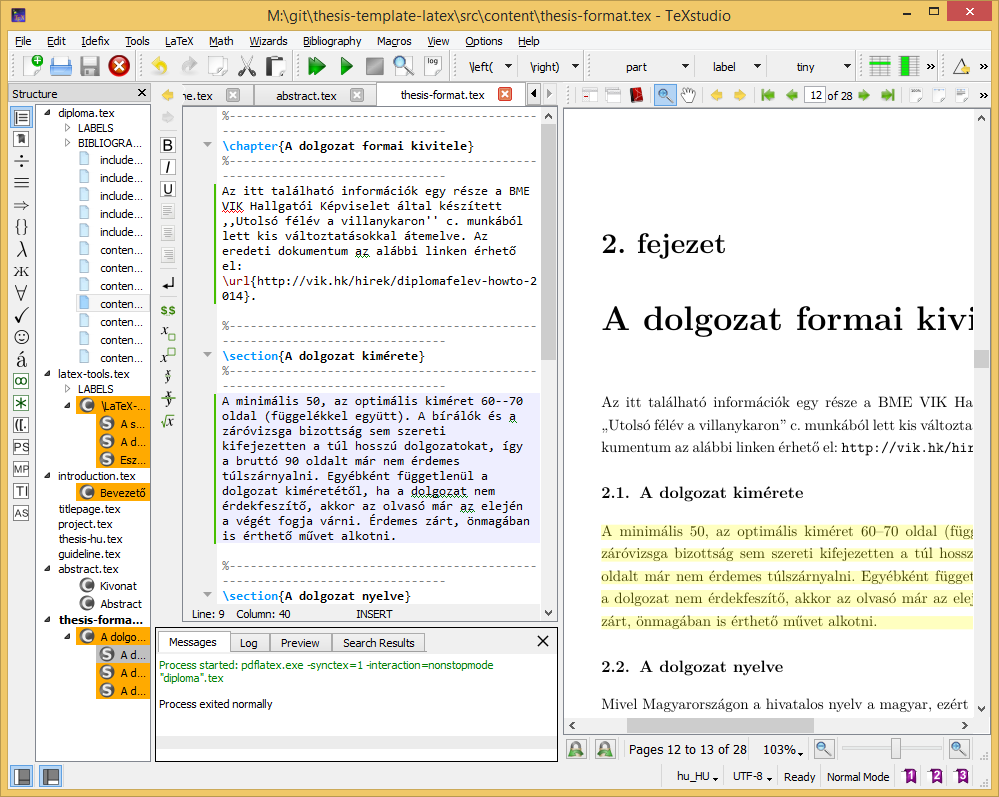
\includegraphics[width=150mm, keepaspectratio]{figures/TeXstudio.png}
\caption{A TeXstudio \LaTeX-szerkesztő.} 
\end{figure}

%----------------------------------------------------------------------------
\clearpage\section{Válasz az ,,Élet, a világmindenség, meg minden'' kérdésére}
%----------------------------------------------------------------------------
A Pitagorasz-tételből levezetve
\begin{align}
c^2=a^2+b^2=42.
\end{align}
A Faraday-indukciós törvényből levezetve
\begin{align}
\rot E=-\frac{dB}{dt}\hspace{1cm}\longrightarrow \hspace{1cm}
U_i=\oint\limits_\mathbf{L}{\mathbf{E}\mathbf{dl}}=-\frac{d}{dt}\int\limits_A{\mathbf{B}\mathbf{da}}=42.
\end{align}


%\label{page:last}
\end{document}
